% ---------------------------------------------------------------------
% EG author guidelines plus sample file for EG publication using LaTeX2e input
% D.Fellner, v1.17, Sep 23, 2010


%\title[Automatic Proxy Geometry Generation]%
%      {Automatic Proxy Geometry Generation}

\title[Automatic Proxy Model Generation]%
      {Hybrid Client/Server Rendering with Automatic Proxy Model Generation}

% for anonymous conference submission please enter your SUBMISSION ID
% instead of the author's name (and leave the affiliation blank) !!
\author[J.\,O. Nygaard \& J. Mikkelsen]
       {J.\,O. Nygaard$^{1}$
        and J. Mikkelsen$^{1}$
        and Husk Anonymisering Hvis Paakrevet! \textbf{JA DET ER DET}$^{1}$
%        S. Spencer$^2$\thanks{Chairman Siggraph Publications Board}
        \\
% For Computer Graphics Forum: Please use the abbreviation of your first name.
%         $^1$SINTEF ICT, applied mathematics, Norway
%        $^2$ Another Department to illustrate the use in papers from authors
%             with different affiliations
       }

% ------------------------------------------------------------------------

% if the Editors-in-Chief have given you the data, you may uncomment
% the following five lines and insert it here
%
% \volume{27}   % the volume in which the issue will be published;
% \issue{1}     % the issue number of the publication
% \pStartPage{1}      % set starting page


%-------------------------------------------------------------------------
\begin{document}

\teaser{
  \centering
  \subfigure[Server-rendered (OpenGL)]{
    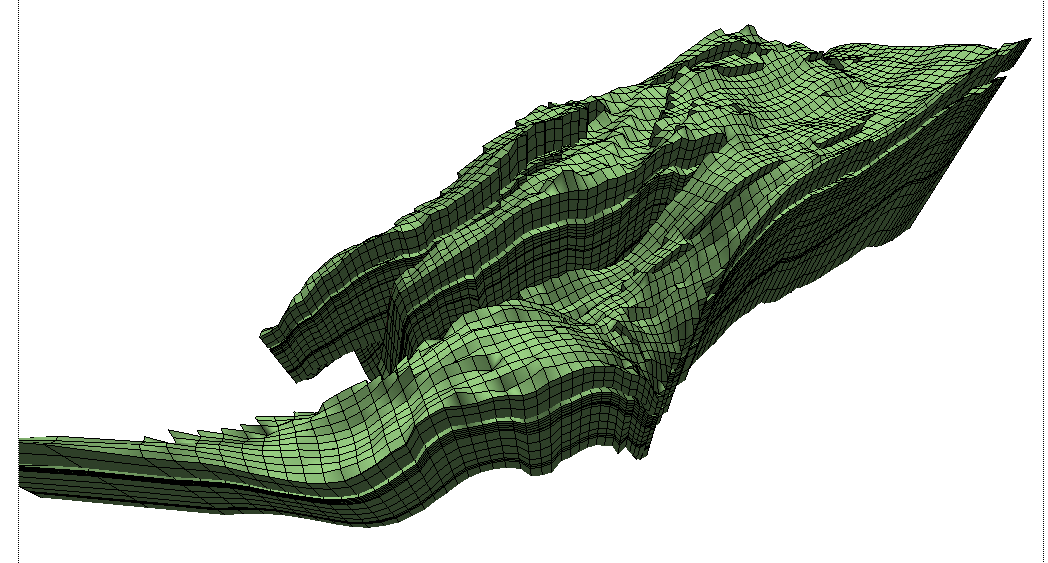
\includegraphics[width=0.3\linewidth, trim={1cm 1cm 1cm 1cm}, clip]{frviewb1.png}
  }
  \subfigure[Client-rendered (WebGL)]{
    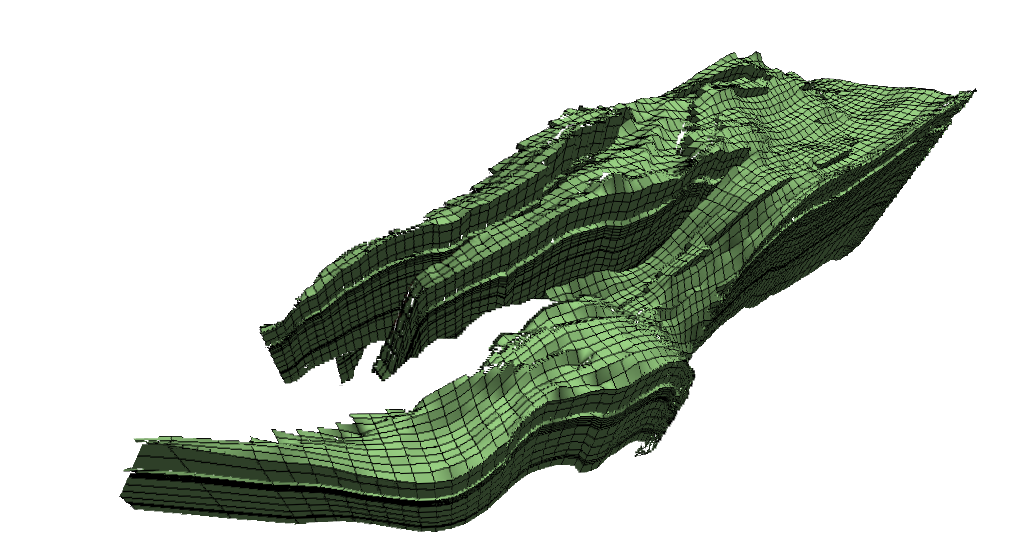
\includegraphics[width=0.3\linewidth, trim={0 1cm 0 1.5cm}, clip]{frviewb2.png}
  }
  \subfigure[Client-rendered (WebGL)]{
    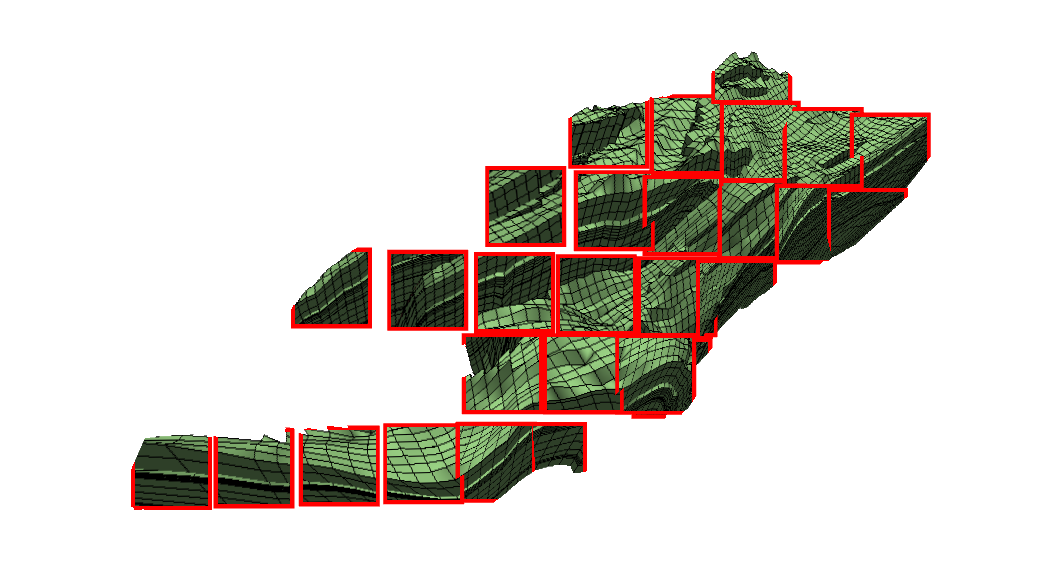
\includegraphics[width=0.3\linewidth, trim={0 1.5cm 0 2cm}, clip]{frviewb3.png}
    % The trim params: left lower right upper
  }
  \caption{\label{fig:FRView} The oil reservoir viewer FRView~\cite{cloudviz},
  showing one server-rendered and two client-rendered images of automatically
  generated and slightly rotated proxy models.  For~(b), parameters are chosen to produce the best
  possible image, and in~(c) we want to highlight artifacts and implementational
  details. See the text for further discussion of these.}
}

\maketitle

\begin{abstract}
\color{red}
   We describe an algorithm and implementation of automatic proxy model
   generation for a client/server remote rendering setup. A {\em proxy model} is
   a light-weight version of a main 3D model that is cheaper to render. We
   automatically derive this from the main model. The client is typically a
   tablet, for which we only assume availability of WebGL and Javascript. The
   server makes use of OpenGL and a web server. When the rate of received
   server-rendered images deteriorate, the client renders the proxy model, which
   is computed from depth buffers bundled with rendered images from the
   server. This algorithm requires little modification of the application
   itself.
   % Husk: Skal vaere en blank linje nedenfor

\begin{classification} % according to http://www.acm.org/class/1998/
\CCScat{Computer Graphics}{I.3.5}{Computational Geometry and Object Modeling}{Geometric algorithms, languages, and systems}
% http://www.acm.org/about/class/ccs98-html
\end{classification}

\end{abstract}




%-------------------------------------------------------------------------
\section{Introduction}

With increasingly powerful rendering engines, in forms ranging from mobile and
hand-held devices to traditional stationary computers, one might be led to
believe that rendering frame rates could only increase and visualization could
only become more interactive. Alas, hand in hand with this development we also
find ever increasing requirements on computational accuracy, power efficiency,
data sizes, scaling, etc.

One effect of this, also enhanced by new cloud-based approaches, wireless
connection, and mobile devices with display capabilities outpacing their
computation and storage capabilities, is that interactivity still is a difficult
issue. In this work, we consider a client/server model for rendering, but this
is just a way of separating the interaction from the rendering; the discussion
also applies to a more integrated setup.  In order to obtain the frame rates on
the client suitable for interactive visualizations, demands are put on
bandwidth, latency and rendering speed. If one or more of these demands are not
met, according to a suitable measure, the frame rate will deteriorate together
with the user experience.

One way to deal with such situations is for the client to have a {\em proxy
model}, defined as a temporary model to be shown and manipulated locally on the
client while waiting for the appropriate image from the server.  A particularly
unwelcomed chore is that of building proxy geometries for various data sets. The
typical ``hello world'' proxy geometry is the familiar bounding box wire frame,
but this will degrade the user experience unacceptably for most
applications. One alternative is to hand craft such simpler proxies. They have
to be simple both for the building cost, and also for the actual rendering on
the possibly very thin client. Another alternative is to automate this process,
a large triangulation may for instance be represented by a much coarser
approximating triangulation that can be built automatically. One disadvantage of
this approach is that this is not easy to do for many kinds of data, like our
main case in which we have an oil reservoir viewer (FRView,~\cite{cloudviz})
that renders large {\em corner point grids}, together with faults, oil wells,
and more. See Figure~\ref{fig:FRView} above for an example of both a fully
completed rendering, and automatically generated proxy geometries rendered in
Google Chrome.

Our suggested solution is to pass depth information from the server along with
ordinary rendered images. From this depth image, a rudimentary 3D model can be
built, and using the ordinary image as a texture, this model can be transformed
and rendered on the client while waiting for the next update from the server. If
the server does not take too long to respond, and/or the client does not change
the position or orientation of the model too much, this display of a proxy model
integrates seemlessly with the slower stream of server-rendered frames.

We also mention that even if bandwidth and latency is not a problem, it may be
desirable to let a server of limited capacity serve many simultaneous users,
hence decreasing the effective server time available for each one. In this case,
suitable scaling properties may still be achieved without increasing server
capacity. The results described in this paper will be commercialized in the new
SINTEF project \mbox{ArrowHead}~\cite{arrowhead}.

\subsection{Previous work}
\label{sec:prevWork}

Our approach has some similarities to {\em image based rendering} (IBR)
techniques, with the difference that an important IBR problem would be the
reconstruction of a depth map from images, while we have access to the full
depth map from a rendering pass.  Another way to use depth maps similar to what
we do, is for ``immersive streaming'', see \eg,~\cite{ibr}, where focus is on
depth map compression, an issue that we also consider. {\color{red}Another work
focused on similar streaming and geometry compression,
is~\cite{teler}. Also,~\cite{220764} contains some of the same ideas as our
work, with respect to image-based rendering accelleration.}

Common to many IBR-algorithms is also that of stitching together 3D or 2.5D
point clouds. We could also in principle do this for our 2.5D maps fetched from
the server, but it is not clear that the benefit would outweight the
cost.

We are not aware of anybody else using depth maps exactly for our purpose, most
research seems to be focused on the retrieval of the depth map from images,
while we use an existing depth map to distill and render temporary geometry.

{\color{red}Finally, we note that these 2.5D heightmaps are exactly what ``3D cameras''
(time-of-flight and other range image sensors) produce, but most authors
considering these are typically building more complex geometries before
visualization.} % , see~\eg,~\cite{}
\marginpar{\textbf{REF?!}}


%-------------------------------------------------------------------------

\section{The auto proxy algorithm}

The main idea is to automatically construct a proxy geometry on the client side
from depth data provided by the server. The server already produces a depth
buffer as part of its rendering process.  This means that our technique is not
immediately ready for \eg, ray-tracing.) This depth buffer may be regarded as a
height map over a viewing plane relative to the observing client. Hence, this
depth map does not contain information about scene elements not in view for the
set of view parameters at the time of server side rendering. Our approach is
based on the assumption that small transformations of this height map still will
give good approximations to the scene being rendered. These renderings are
exactly what the client will compute and show while waiting for the next update
from the server. See Figure~\ref{fig:2Dheightmap} and
Figure~\ref{fig:2DheightmapRotated} below for an illustration of this heightmap
computed on the server, and a recovered 3D model on the client.

\begin{figure}[htb]
  \centering
  \begin{tikzpicture}[scale=0.5, >=triangle 45] % , show background rectangle]


%  \node[scale=0.15, above right] (screenshotcenter) at (0,0) {\includegraphics{test.jpg}};
%  \coordinate (widthheight) at ($2*(screenshotcenter)$);

%  \draw [fill, circle, inner sep=0pt, minimum size=3pt, color=black] (0, 0) circle (3pt);
%  \draw [fill, circle, inner sep=0pt, minimum size=3pt, color=red] (screenshotcenter) circle (3pt);

%  \draw let
%    \p1 = ( $ 2*(screenshotcenter) $ )
%  in
%    [fill=none] (0, 0) rectangle (\x1, \y1);


%  \newcommand\expansion{0.5}
%  \coordinate (lowerleft)        at ( $ (0, 0) - \expansion*(widthheight) $ );
%  \coordinate (upperright)       at ( $ (widthheight) + \expansion*(widthheight) $ );
  
%  \draw [fill=none] (lowerleft) rectangle (upperright);

  % View frustum
  \fill[fill=gray!10] (1, 0.7) -- (9, 0.7) -- (10, 4.3) -- (0, 4.3) -- cycle;

  % Some scene
  \draw[red, line width=3pt] (2, 3) -- (5, 2);
  \draw[green, line width=3pt] (5, 2) -- (8, 4);


  % Corresponding pixels and depth fragments
  \def \pixelwidth  {0.4}
  \def \pixelheight {0.3}
  \def \redstart    {2.2}
  \def \redpixels   {7}
  \def \pixels      {13}
  \foreach \s in {1, ..., \pixels} {
    \def \x { \redstart + \s * \pixelwidth }
    \def \xx { \x + \pixelwidth }
    \ifthenelse{\s < \redpixels} {
      \draw[red, fill=red!50] (\x, 1) rectangle (\xx, 1+\pixelheight); 
    } {
      \draw[green, fill=green!50] (\x, 1) rectangle (\xx, 1+\pixelheight);
    }
    \pgfmathsetmacro\depthcol{abs(\redpixels-0.5-\s) * 25}
    \draw[black, fill=gray!\depthcol] (\x, 1+\pixelheight) rectangle (\xx, 1+2*\pixelheight);
  }


%\def \n {5}
%\def \radius {3cm}
%\def \margin {8} % margin in angles, depends on the radius
%\foreach \s in {1,...,\n}
%{
%  \node[draw, circle] at ({360/\n * (\s - 1)}:\radius) {$\s$};
%  \draw[->, >=latex] ({360/\n * (\s - 1)+\margin}:\radius) 
%    arc ({360/\n * (\s - 1)+\margin}:{360/\n * (\s)-\margin}:\radius);
%}



  % Indicated nodes and intersections
%  \draw [fill, circle, inner sep=0pt, minimum size=3pt, color=black] (T0) circle (3pt);

  % Labels
%  \draw (T0) node[black, scale=0.8, shift={(0, -2ex)}] {$\Tv_0$};


\end{tikzpicture}

  \caption{\label{fig:2Dheightmap} The rendered image (of \eg, a cube) as a
           height map seen from above, for a certain transformation. Also shown
           are the corresponding RGB-fragments (red and green) and depth
           fragments (floating point scalars shown as grayscale pixels.)}
\end{figure}

In Figure~\ref{fig:2DheightmapRotated} below, a sequence of three server-rendered
images (solid lines, red and blue) is shown, together with intermediate
client-rendered proxy models with different features. These features will be
discussed later, in Section~\ref{sec:client}.

\begin{figure}[htb]
  \centering
  \subfigure[Low frame rate]{
    %\begin{tikzpicture}[ scale=.25, show background rectangle]
\begin{tikzpicture}[scale=0.32, >=triangle 45, show background rectangle,
  declare function = {
    rotx(\x,\y,\th) = cos(\th)*\x - sin(\th)*\y; % NB! Cannot have space between parameters it seems!
    roty(\x,\y,\th) = sin(\th)*\x + cos(\th)*\y;
  }
  ]

  % View frustum
  \fill[fill=gray!20] (1, 0) -- (9, 0) -- (10, 5) -- (0, 5) -- cycle;
  % \clip (1, 0) -- (9, 0) -- (10, 5) -- (0, 5) -- cycle;
  % Clipping looks ok, but clipped content still expands bbox!! Solving this by reducing \pixels below from 13 to 11...


  % Defining some figure params

  \def \pixelwidth  {0.4}
  \def \pixelheight {0.3}
  \def \redstart    {2.2}
  \def \redpixels   {5}
  \def \pixels      {11}
  \def \linewidth   {1.25pt}
  \def \theta       {25}
  \def \cx          {5}
  \def \cy          {3}
  \def \rightcol    {red!100}
  \def \leftcolL    {blue!100}
  %\def \leftcolR    {red!100!blue!0} % Why doesn't this work?! (The color becomes white)
  \def \leftcolR    {red!100}


  % The scene, using same coordinate calculations as in the loop below

  \foreach \t in {0, ..., 4} {

    \pgfmathsetmacro\theta{25*\t}

    \ifthenelse{ \t = 0 \OR \t = 2 \OR \t = 4} {
      \def \rightcolToUse {\rightcol}
      \def \leftcolLToUse {\leftcolL}
      \def \leftcolRToUse {\leftcolR}
    }{
      \def \rightcolToUse {red!10}
      \def \leftcolLToUse {blue!10}
      \def \leftcolRToUse {red!10}
    }

    \pgfmathsetmacro\s{1}
    \pgfmathsetmacro\posx{0.5*(\s-1) + 2}
    \pgfmathsetmacro\posy{3.5 - 0.6*(\s-1)}
    \pgfmathsetmacro\posxRot{rotx(\posx-\cx, \posy-\cy, \theta)+\cx}
    \pgfmathsetmacro\posyRot{roty(\posx-\cx, \posy-\cy, \theta)+\cy}
    \coordinate (left) at ( \posxRot, \posyRot );
    
    \pgfmathsetmacro\s{\redpixels - 1}
    \pgfmathsetmacro\posx{0.5*(\s-1) + 2}
    \pgfmathsetmacro\posy{3.5 - 0.6*(\s-1)}
    \pgfmathsetmacro\posxRot{rotx(\posx-\cx, \posy-\cy, \theta)+\cx}
    \pgfmathsetmacro\posyRot{roty(\posx-\cx, \posy-\cy, \theta)+\cy}
    \coordinate (middle) at ( \posxRot, \posyRot );
    
    % The offset necessary for the red and green lines to meet properly
    \pgfmathsetmacro\redgreenintersection{3.5 -(0.6+0.2)*(\s-1)}
    
    \pgfmathsetmacro\s{\pixels}
    \pgfmathsetmacro\posx{0.5*(\s-1) + 2}
    \pgfmathsetmacro\posy{0.2*(\s-1) + \redgreenintersection}
    \pgfmathsetmacro\posxRot{rotx(\posx-\cx, \posy-\cy, \theta)+\cx}
    \pgfmathsetmacro\posyRot{roty(\posx-\cx, \posy-\cy, \theta)+\cy}
    \coordinate (right) at ( \posxRot, \posyRot );
    
    % The "server-rendered model"
    \fill[left color=\leftcolLToUse, right color=\leftcolRToUse, draw=none]
    (left) -- (middle) -- +(0, 3*\linewidth) -- ($ (left) + (0, 3*\linewidth) $) -- cycle;
    % Why is the factor 3 needed here?!?!
    % And why is there a (very thin) border?
    % And why is it not equally thick everywhere?

    \draw[\rightcolToUse, line width=\linewidth] (middle) -- (right);

  }


\end{tikzpicture}

  }
  \subfigure[Initial proxy model]{
    \begin{tikzpicture}[scale=0.32, >=triangle 45, show background rectangle,
  declare function = {
    rotx(\x,\y,\th) = cos(\th)*\x - sin(\th)*\y; % NB! Cannot have space between parameters it seems!
    roty(\x,\y,\th) = sin(\th)*\x + cos(\th)*\y;
  }
  ]

  % View frustum
  \fill[fill=gray!20] (1, 0) -- (9, 0) -- (10, 5) -- (0, 5) -- cycle;


  % Defining some figure params

  \def \pixelwidth  {0.4}
  \def \pixelheight {0.3}
  \def \redstart    {2.2}
  \def \redpixels   {5}
  \def \pixels      {11}
  \def \linewidth   {1.25pt}
  \def \cx          {5}
  \def \cy          {2.5}

  \pgfmathsetmacro\halfpixelwidth{0.5*\pixelwidth}


  \foreach \frame in {0} {  % , ..., 4} {
    \pgfmathsetmacro\theta{25*\frame}

    \ifthenelse{ \frame = 0 \OR \frame = 2 \OR \frame = 4} {
      \def \rightcolToUse {red!100}
      \def \leftcolLToUse {blue!100}
      \def \leftcolRToUse {red!100}
    }{
      \def \rightcolToUse {red!10}
      \def \leftcolLToUse {blue!10}
      \def \leftcolRToUse {red!10}
    }
    
    \def \withSplats {1}
    \def \withLargeSplats {0}
    \def \withConstantWidthSplats {1}
    \def \withFragDepth {0}

        \pgfmathsetmacro\s{1}
    \pgfmathsetmacro\posx{0.5*(\s-1) + 2}
    \pgfmathsetmacro\posy{3.5 - 0.6*(\s-1)}
    \pgfmathsetmacro\posxRot{rotx(\posx-\cx, \posy-\cy, 0)+\cx}
    \pgfmathsetmacro\posyRot{roty(\posx-\cx, \posy-\cy, 0)+\cy}
    \coordinate (left) at ( \posxRot, \posyRot );
    
    \pgfmathsetmacro\s{\redpixels - 1}
    \pgfmathsetmacro\posx{0.5*(\s-1) + 2}
    \pgfmathsetmacro\posy{3.5 - 0.6*(\s-1)}
    \pgfmathsetmacro\posxRot{rotx(\posx-\cx, \posy-\cy, 0)+\cx}
    \pgfmathsetmacro\posyRot{roty(\posx-\cx, \posy-\cy, 0)+\cy}
    \coordinate (middle) at ( \posxRot, \posyRot );
    
    % The offset necessary for the red and green lines to meet properly
    \pgfmathsetmacro\redgreenintersection{3.5 -(0.6+0.2)*(\s-1)}
    
    \pgfmathsetmacro\s{\pixels}
    \pgfmathsetmacro\posx{0.5*(\s-1) + 2}
    \pgfmathsetmacro\posy{0.2*(\s-1) + \redgreenintersection}
    \pgfmathsetmacro\posxRot{rotx(\posx-\cx, \posy-\cy, 0)+\cx}
    \pgfmathsetmacro\posyRot{roty(\posx-\cx, \posy-\cy, 0)+\cy}
    \coordinate (right) at ( \posxRot, \posyRot );
    
    % The "server-rendered model"
    \fill[left color=\leftcolLToUse, right color=\leftcolRToUse, draw=none]
      (left) -- (middle) -- +(0, 5*\linewidth) -- ($ (left) + (0, 5*\linewidth) $) -- cycle;
    % Why is the factor 3 needed here?!?!
    % And why is there a (very thin) border?
    % And why is it not equally thick everywhere?
    \draw[\rightcolToUse, line width=\linewidth] (middle) -- (right);

    \ifthenelse{ \withSplats = 1 } {
      \foreach \s in {1, ..., \pixels} {
        \ifthenelse{\s < \redpixels} {
          \pgfmathsetmacro\posx{0.5*(\s-1) + 2}
          \pgfmathsetmacro\posy{3.5 - 0.6*(\s-1)}
          \pgfmathsetmacro\posxRot{rotx(\posx-\cx, \posy-\cy, \theta)+\cx}
          \pgfmathsetmacro\posyRot{roty(\posx-\cx, \posy-\cy, \theta)+\cy}
          
          % Screen-space-sized splats
          \pgfmathsetmacro\posx{0.5*(\s-1-1) + 2}
          \pgfmathsetmacro\posy{3.5 - 0.6*(\s-1-1)}
          \pgfmathsetmacro\posxRotL{rotx(\posx-\cx, \posy-\cy, \theta)+\cx}
          \pgfmathsetmacro\posyRotL{roty(\posx-\cx, \posy-\cy, \theta)+\cy}
          \pgfmathsetmacro\posx{0.5*(\s-1) + 2}
          \pgfmathsetmacro\posy{3.5 - 0.6*(\s-1)}
          \pgfmathsetmacro\posxRotR{rotx(\posx-\cx, \posy-\cy, \theta)+\cx}
          \pgfmathsetmacro\posyRotR{roty(\posx-\cx, \posy-\cy, \theta)+\cy}
          \pgfmathsetmacro\halfWidthToUse{0.5*(\posxRotR-\posxRotL)}
          
          % Overriding with constant width for one of the sub-figures
          \ifthenelse{ \withConstantWidthSplats = 1 } {
            \pgfmathsetmacro\halfWidthToUse{\halfpixelwidth}
          }{}

          \ifthenelse{ \withLargeSplats = 1 } {
            % Varying color here on the left side
            \pgfmathsetmacro\tl{100*(\s-1)/\redpixels}
            \pgfmathsetmacro\ul{100-\tl)}
            \pgfmathsetmacro\tr{100*(\s  )/\redpixels}
            \pgfmathsetmacro\ur{100-\tr}
            \ifthenelse{ \withFragDepth = 0 } {
              \draw[left color=red!\tl!blue!\ul, right color=red!\tr!blue!\ur]
                (\posxRot-\halfWidthToUse, \posyRot) rectangle +(2*\halfWidthToUse, 0.2);
            }{
              % Tror kanskje at problemet med at ting kommer for langt til venstre her, skyldes at vi ser paa 
              % linjestykker fra s-1-1 til s-1. Burde muligens vaert fra s-1-0.5 til s-1+0.5?!
              % Replace with rotated rectangles, will probably look better...
              \draw[left color=red!\tl!blue!\ul, right color=red!\tr!blue!\ur]
                (\posxRotL, \posyRotL) -- (\posxRotR, \posyRotR) -- +(0, 5*\linewidth) -- 
                ($ (\posxRotL, \posyRotL) + (0, 5*\linewidth) $) -- cycle;
            }
          }{
            % Constant color, just a dot
            \pgfmathsetmacro\t{100*\s/\redpixels}
            \pgfmathsetmacro\u{100*(1.0-\s/\redpixels)}
            \draw[fill=red!\t!blue!\u] (\posxRot, \posyRot) circle(0.15);
          }
        } {
          \pgfmathsetmacro\posx{0.5*(\s-1) + 2}
          \pgfmathsetmacro\posy{0.2*(\s-1) + \redgreenintersection}
          \pgfmathsetmacro\posxRot{rotx(\posx-\cx, \posy-\cy, \theta)+\cx}
          \pgfmathsetmacro\posyRot{roty(\posx-\cx, \posy-\cy, \theta)+\cy}
          
          % Screen-space-sized splats
          \pgfmathsetmacro\posx{0.5*(\s-1-1) + 2}
          \pgfmathsetmacro\posy{0.2*(\s-1-1) + \redgreenintersection}
          \pgfmathsetmacro\posxRotL{rotx(\posx-\cx, \posy-\cy, \theta)+\cx}
          \pgfmathsetmacro\posyRotL{roty(\posx-\cx, \posy-\cy, \theta)+\cy}
          \pgfmathsetmacro\posx{0.5*(\s-1) + 2}
          \pgfmathsetmacro\posy{0.2*(\s-1) + \redgreenintersection}
          \pgfmathsetmacro\posxRotR{rotx(\posx-\cx, \posy-\cy, \theta)+\cx}
          \pgfmathsetmacro\posyRotR{roty(\posx-\cx, \posy-\cy, \theta)+\cy}
          \pgfmathsetmacro\halfWidthToUse{0.5*(\posxRotR-\posxRotL)}
          
          \ifthenelse{ \withConstantWidthSplats = 1 } {
            % Overriding with constant width for one of the sub-figures
            \pgfmathsetmacro\halfWidthToUse{\halfpixelwidth}
          }{}

          \ifthenelse{ \withLargeSplats = 1 } {
            \ifthenelse{ \withFragDepth = 0 } {
              \draw[fill=\rightcolToUse]
                (\posxRot-\halfWidthToUse, \posyRot) rectangle +(2*\halfWidthToUse, 0.2);
            }{
              % \draw[fill=\rightcolToUse, line width=1.5pt] (\posxRotL, \posyRotL) -- (\posxRotR, \posyRotR);
              % Tror kanskje at problemet med at ting kommer for langt til venstre her, skyldes at vi ser paa 
              % linjestykker fra s-1-1 til s-1. Burde muligens vaert fra s-1-0.5 til s-1+0.5?!
              % Replace with rotated rectangles, will probably look better...
              \draw[fill=\rightcolToUse]
                (\posxRotL, \posyRotL) -- (\posxRotR, \posyRotR) -- +(0, 5*\linewidth) -- 
                ($ (\posxRotL, \posyRotL) + (0, 5*\linewidth) $) -- cycle;
            }
          }{
            % Constant color, just a dot
            \draw[fill=\rightcolToUse] (\posxRot, \posyRot) circle(0.15);
          }
        }
      }
    }{}

    
  }


\end{tikzpicture}

  }
  \subfigure[Client-generated frame]{
    \begin{tikzpicture}[scale=0.32, >=triangle 45, show background rectangle,
  declare function = {
    rotx(\x,\y,\th) = cos(\th)*\x - sin(\th)*\y; % NB! Cannot have space between parameters it seems!
    roty(\x,\y,\th) = sin(\th)*\x + cos(\th)*\y;
  }
  ]

  % View frustum
  \fill[fill=gray!20] (1, 0) -- (9, 0) -- (10, 5) -- (0, 5) -- cycle;


  % Defining some figure params

  \def \pixelwidth  {0.5}
  \def \pixelheight {0.3}
  \def \redstart    {2.2}
  \def \redpixels   {5}
  \def \pixels      {11}
  \def \linewidth   {1.25pt}
  \def \theta       {25}        % Degrees
  \def \cx          {5}
  \def \cy          {2.5}

  \pgfmathsetmacro\halfpixelwidth{0.5*\pixelwidth}


  \foreach \frame in {0, ..., 1} {  % , ..., 4} {
    \pgfmathsetmacro\theta{25*\frame}

    \def \rightcolToUse {red!100}
    \def \leftcolLToUse {blue!100}
    \def \leftcolRToUse {red!100}

    \ifthenelse{ \frame = 0 } {
      \def \withSplats {0}
    }{
      \def \withSplats {1}
    }
    \def \withLargeSplats {0}
    \def \withConstantWidthSplats {1}
    \def \withFragDepth {0}

        \pgfmathsetmacro\s{1}
    \pgfmathsetmacro\posx{0.5*(\s-1) + 2}
    \pgfmathsetmacro\posy{3.5 - 0.6*(\s-1)}
    \pgfmathsetmacro\posxRot{rotx(\posx-\cx, \posy-\cy, 0)+\cx}
    \pgfmathsetmacro\posyRot{roty(\posx-\cx, \posy-\cy, 0)+\cy}
    \coordinate (left) at ( \posxRot, \posyRot );
    
    \pgfmathsetmacro\s{\redpixels - 1}
    \pgfmathsetmacro\posx{0.5*(\s-1) + 2}
    \pgfmathsetmacro\posy{3.5 - 0.6*(\s-1)}
    \pgfmathsetmacro\posxRot{rotx(\posx-\cx, \posy-\cy, 0)+\cx}
    \pgfmathsetmacro\posyRot{roty(\posx-\cx, \posy-\cy, 0)+\cy}
    \coordinate (middle) at ( \posxRot, \posyRot );
    
    % The offset necessary for the red and green lines to meet properly
    \pgfmathsetmacro\redgreenintersection{3.5 -(0.6+0.2)*(\s-1)}
    
    \pgfmathsetmacro\s{\pixels}
    \pgfmathsetmacro\posx{0.5*(\s-1) + 2}
    \pgfmathsetmacro\posy{0.2*(\s-1) + \redgreenintersection}
    \pgfmathsetmacro\posxRot{rotx(\posx-\cx, \posy-\cy, 0)+\cx}
    \pgfmathsetmacro\posyRot{roty(\posx-\cx, \posy-\cy, 0)+\cy}
    \coordinate (right) at ( \posxRot, \posyRot );
    
    % The "server-rendered model"
    \fill[left color=\leftcolLToUse, right color=\leftcolRToUse, draw=none]
      (left) -- (middle) -- +(0, 5*\linewidth) -- ($ (left) + (0, 5*\linewidth) $) -- cycle;
    % Why is the factor 3 needed here?!?!
    % And why is there a (very thin) border?
    % And why is it not equally thick everywhere?
    \draw[\rightcolToUse, line width=\linewidth] (middle) -- (right);

    \ifthenelse{ \withSplats = 1 } {
      \foreach \s in {1, ..., \pixels} {
        \ifthenelse{\s < \redpixels} {
          \pgfmathsetmacro\posx{0.5*(\s-1) + 2}
          \pgfmathsetmacro\posy{3.5 - 0.6*(\s-1)}
          \pgfmathsetmacro\posxRot{rotx(\posx-\cx, \posy-\cy, \theta)+\cx}
          \pgfmathsetmacro\posyRot{roty(\posx-\cx, \posy-\cy, \theta)+\cy}
          
          % Screen-space-sized splats
          \pgfmathsetmacro\posx{0.5*(\s-1-1) + 2}
          \pgfmathsetmacro\posy{3.5 - 0.6*(\s-1-1)}
          \pgfmathsetmacro\posxRotL{rotx(\posx-\cx, \posy-\cy, \theta)+\cx}
          \pgfmathsetmacro\posyRotL{roty(\posx-\cx, \posy-\cy, \theta)+\cy}
          \pgfmathsetmacro\posx{0.5*(\s-1) + 2}
          \pgfmathsetmacro\posy{3.5 - 0.6*(\s-1)}
          \pgfmathsetmacro\posxRotR{rotx(\posx-\cx, \posy-\cy, \theta)+\cx}
          \pgfmathsetmacro\posyRotR{roty(\posx-\cx, \posy-\cy, \theta)+\cy}
          \pgfmathsetmacro\halfWidthToUse{0.5*(\posxRotR-\posxRotL)}
          
          % Overriding with constant width for one of the sub-figures
          \ifthenelse{ \withConstantWidthSplats = 1 } {
            \pgfmathsetmacro\halfWidthToUse{\halfpixelwidth}
          }{}

          \ifthenelse{ \withLargeSplats = 1 } {
            % Varying color here on the left side
            \pgfmathsetmacro\tl{100*(\s-1)/\redpixels}
            \pgfmathsetmacro\ul{100-\tl)}
            \pgfmathsetmacro\tr{100*(\s  )/\redpixels}
            \pgfmathsetmacro\ur{100-\tr}
            \ifthenelse{ \withFragDepth = 0 } {
              \draw[left color=red!\tl!blue!\ul, right color=red!\tr!blue!\ur]
                (\posxRot-\halfWidthToUse, \posyRot) rectangle +(2*\halfWidthToUse, 0.2);
            }{
              % Tror kanskje at problemet med at ting kommer for langt til venstre her, skyldes at vi ser paa 
              % linjestykker fra s-1-1 til s-1. Burde muligens vaert fra s-1-0.5 til s-1+0.5?!
              % Replace with rotated rectangles, will probably look better...
              \draw[left color=red!\tl!blue!\ul, right color=red!\tr!blue!\ur]
                (\posxRotL, \posyRotL) -- (\posxRotR, \posyRotR) -- +(0, 5*\linewidth) -- 
                ($ (\posxRotL, \posyRotL) + (0, 5*\linewidth) $) -- cycle;
            }
          }{
            % Constant color, just a dot
            \pgfmathsetmacro\t{100*\s/\redpixels}
            \pgfmathsetmacro\u{100*(1.0-\s/\redpixels)}
            \draw[fill=red!\t!blue!\u] (\posxRot, \posyRot) circle(0.15);
          }
        } {
          \pgfmathsetmacro\posx{0.5*(\s-1) + 2}
          \pgfmathsetmacro\posy{0.2*(\s-1) + \redgreenintersection}
          \pgfmathsetmacro\posxRot{rotx(\posx-\cx, \posy-\cy, \theta)+\cx}
          \pgfmathsetmacro\posyRot{roty(\posx-\cx, \posy-\cy, \theta)+\cy}
          
          % Screen-space-sized splats
          \pgfmathsetmacro\posx{0.5*(\s-1-1) + 2}
          \pgfmathsetmacro\posy{0.2*(\s-1-1) + \redgreenintersection}
          \pgfmathsetmacro\posxRotL{rotx(\posx-\cx, \posy-\cy, \theta)+\cx}
          \pgfmathsetmacro\posyRotL{roty(\posx-\cx, \posy-\cy, \theta)+\cy}
          \pgfmathsetmacro\posx{0.5*(\s-1) + 2}
          \pgfmathsetmacro\posy{0.2*(\s-1) + \redgreenintersection}
          \pgfmathsetmacro\posxRotR{rotx(\posx-\cx, \posy-\cy, \theta)+\cx}
          \pgfmathsetmacro\posyRotR{roty(\posx-\cx, \posy-\cy, \theta)+\cy}
          \pgfmathsetmacro\halfWidthToUse{0.5*(\posxRotR-\posxRotL)}
          
          \ifthenelse{ \withConstantWidthSplats = 1 } {
            % Overriding with constant width for one of the sub-figures
            \pgfmathsetmacro\halfWidthToUse{\halfpixelwidth}
          }{}

          \ifthenelse{ \withLargeSplats = 1 } {
            \ifthenelse{ \withFragDepth = 0 } {
              \draw[fill=\rightcolToUse]
                (\posxRot-\halfWidthToUse, \posyRot) rectangle +(2*\halfWidthToUse, 0.2);
            }{
              % \draw[fill=\rightcolToUse, line width=1.5pt] (\posxRotL, \posyRotL) -- (\posxRotR, \posyRotR);
              % Tror kanskje at problemet med at ting kommer for langt til venstre her, skyldes at vi ser paa 
              % linjestykker fra s-1-1 til s-1. Burde muligens vaert fra s-1-0.5 til s-1+0.5?!
              % Replace with rotated rectangles, will probably look better...
              \draw[fill=\rightcolToUse]
                (\posxRotL, \posyRotL) -- (\posxRotR, \posyRotR) -- +(0, 5*\linewidth) -- 
                ($ (\posxRotL, \posyRotL) + (0, 5*\linewidth) $) -- cycle;
            }
          }{
            % Constant color, just a dot
            \draw[fill=\rightcolToUse] (\posxRot, \posyRot) circle(0.15);
          }
        }
      }
    }{}

    
  }
  

\end{tikzpicture}

  }
  \subfigure[With texturing]{
    \begin{tikzpicture}[scale=0.32, >=triangle 45, % show background rectangle,
  declare function = {
    rotx(\x,\y,\th) = cos(\th)*\x - sin(\th)*\y; % NB! Cannot have space between parameters it seems!
    roty(\x,\y,\th) = sin(\th)*\x + cos(\th)*\y;
  }
  ]

  % View frustum
\fill[fill=gray!10] (1, 0) -- (9, 0) -- (10, 5) -- (0, 5) -- cycle;

% \clip (1, 0) -- (9, 0) -- (10, 5) -- (0, 5) -- cycle;

% Clipping looks ok, but clipped content still expands bbox!! Solving this by
% reducing \pixels below from 13 to 11...


% Defining some figure params

\def \pixelwidth  {0.5}
\def \pixelheight {0.3}
\def \theta       {25}        % Degrees
%\def \pixelwidth  {0.4}
%\def \pixelheight {0.3}
\def \redstart    {2.2}
\def \redpixels   {5}
\def \pixels      {12}
\def \linewidth   {1.25pt}
\def \cx          {5}
\def \cy          {2.5}

% bare for fig3a.tex: ?
\def \rightcol    {red!100}
\def \leftcolL    {blue!100}
%\def \leftcolR    {red!100!blue!0} % Why doesn't this work?! (The color becomes white)
\def \leftcolR    {red!100}

\pgfmathsetmacro\halfpixelwidth{0.5*\pixelwidth}


  \foreach \frame in {0, ..., 1} {
    \pgfmathsetmacro\theta{25*\frame}

    \def \rightcolToUse {red!100}
    \def \leftcolLToUse {blue!100}
    \def \leftcolRToUse {red!100}

    \ifthenelse{ \frame = 0 } {
      \def \withSplats {0}
    }{
      \def \withSplats {1}
    }
    \def \withLargeSplats {1}
    \def \withConstantWidthSplats {1}
    \def \withFragDepth {0}

        \pgfmathsetmacro\s{1}
    \pgfmathsetmacro\posx{0.5*(\s-1) + 2}
    \pgfmathsetmacro\posy{3.5 - 0.6*(\s-1)}
    \pgfmathsetmacro\posxRot{rotx(\posx-\cx, \posy-\cy, 0)+\cx}
    \pgfmathsetmacro\posyRot{roty(\posx-\cx, \posy-\cy, 0)+\cy}
    \coordinate (left) at ( \posxRot, \posyRot );
    
    \pgfmathsetmacro\s{\redpixels - 1}
    \pgfmathsetmacro\posx{0.5*(\s-1) + 2}
    \pgfmathsetmacro\posy{3.5 - 0.6*(\s-1)}
    \pgfmathsetmacro\posxRot{rotx(\posx-\cx, \posy-\cy, 0)+\cx}
    \pgfmathsetmacro\posyRot{roty(\posx-\cx, \posy-\cy, 0)+\cy}
    \coordinate (middle) at ( \posxRot, \posyRot );
    
    % The offset necessary for the red and green lines to meet properly
    \pgfmathsetmacro\redgreenintersection{3.5 -(0.6+0.2)*(\s-1)}
    
    \pgfmathsetmacro\s{\pixels}
    \pgfmathsetmacro\posx{0.5*(\s-1) + 2}
    \pgfmathsetmacro\posy{0.2*(\s-1) + \redgreenintersection}
    \pgfmathsetmacro\posxRot{rotx(\posx-\cx, \posy-\cy, 0)+\cx}
    \pgfmathsetmacro\posyRot{roty(\posx-\cx, \posy-\cy, 0)+\cy}
    \coordinate (right) at ( \posxRot, \posyRot );
    
    % The "server-rendered model"
    \fill[left color=\leftcolLToUse, right color=\leftcolRToUse, draw=none]
      (left) -- (middle) -- +(0, 5*\linewidth) -- ($ (left) + (0, 5*\linewidth) $) -- cycle;
    % Why is the factor 3 needed here?!?!
    % And why is there a (very thin) border?
    % And why is it not equally thick everywhere?
    \draw[\rightcolToUse, line width=\linewidth] (middle) -- (right);

    \ifthenelse{ \withSplats = 1 } {
      \foreach \s in {1, ..., \pixels} {
        \ifthenelse{\s < \redpixels} {
          \pgfmathsetmacro\posx{0.5*(\s-1) + 2}
          \pgfmathsetmacro\posy{3.5 - 0.6*(\s-1)}
          \pgfmathsetmacro\posxRot{rotx(\posx-\cx, \posy-\cy, \theta)+\cx}
          \pgfmathsetmacro\posyRot{roty(\posx-\cx, \posy-\cy, \theta)+\cy}
          
          % Screen-space-sized splats
          \pgfmathsetmacro\posx{0.5*(\s-1-1) + 2}
          \pgfmathsetmacro\posy{3.5 - 0.6*(\s-1-1)}
          \pgfmathsetmacro\posxRotL{rotx(\posx-\cx, \posy-\cy, \theta)+\cx}
          \pgfmathsetmacro\posyRotL{roty(\posx-\cx, \posy-\cy, \theta)+\cy}
          \pgfmathsetmacro\posx{0.5*(\s-1) + 2}
          \pgfmathsetmacro\posy{3.5 - 0.6*(\s-1)}
          \pgfmathsetmacro\posxRotR{rotx(\posx-\cx, \posy-\cy, \theta)+\cx}
          \pgfmathsetmacro\posyRotR{roty(\posx-\cx, \posy-\cy, \theta)+\cy}
          \pgfmathsetmacro\halfWidthToUse{0.5*(\posxRotR-\posxRotL)}
          
          % Overriding with constant width for one of the sub-figures
          \ifthenelse{ \withConstantWidthSplats = 1 } {
            \pgfmathsetmacro\halfWidthToUse{\halfpixelwidth}
          }{}

          \ifthenelse{ \withLargeSplats = 1 } {
            % Varying color here on the left side
            \pgfmathsetmacro\tl{100*(\s-1)/\redpixels}
            \pgfmathsetmacro\ul{100-\tl)}
            \pgfmathsetmacro\tr{100*(\s  )/\redpixels}
            \pgfmathsetmacro\ur{100-\tr}
            \ifthenelse{ \withFragDepth = 0 } {
              \draw[left color=red!\tl!blue!\ul, right color=red!\tr!blue!\ur]
                (\posxRot-\halfWidthToUse, \posyRot) rectangle +(2*\halfWidthToUse, 0.2);
            }{
              % Tror kanskje at problemet med at ting kommer for langt til venstre her, skyldes at vi ser paa 
              % linjestykker fra s-1-1 til s-1. Burde muligens vaert fra s-1-0.5 til s-1+0.5?!
              % Replace with rotated rectangles, will probably look better...
              \draw[left color=red!\tl!blue!\ul, right color=red!\tr!blue!\ur]
                (\posxRotL, \posyRotL) -- (\posxRotR, \posyRotR) -- +(0, 5*\linewidth) -- 
                ($ (\posxRotL, \posyRotL) + (0, 5*\linewidth) $) -- cycle;
            }
          }{
            % Constant color, just a dot
            \pgfmathsetmacro\t{100*\s/\redpixels}
            \pgfmathsetmacro\u{100*(1.0-\s/\redpixels)}
            \draw[fill=red!\t!blue!\u] (\posxRot, \posyRot) circle(0.15);
          }
        } {
          \pgfmathsetmacro\posx{0.5*(\s-1) + 2}
          \pgfmathsetmacro\posy{0.2*(\s-1) + \redgreenintersection}
          \pgfmathsetmacro\posxRot{rotx(\posx-\cx, \posy-\cy, \theta)+\cx}
          \pgfmathsetmacro\posyRot{roty(\posx-\cx, \posy-\cy, \theta)+\cy}
          
          % Screen-space-sized splats
          \pgfmathsetmacro\posx{0.5*(\s-1-1) + 2}
          \pgfmathsetmacro\posy{0.2*(\s-1-1) + \redgreenintersection}
          \pgfmathsetmacro\posxRotL{rotx(\posx-\cx, \posy-\cy, \theta)+\cx}
          \pgfmathsetmacro\posyRotL{roty(\posx-\cx, \posy-\cy, \theta)+\cy}
          \pgfmathsetmacro\posx{0.5*(\s-1) + 2}
          \pgfmathsetmacro\posy{0.2*(\s-1) + \redgreenintersection}
          \pgfmathsetmacro\posxRotR{rotx(\posx-\cx, \posy-\cy, \theta)+\cx}
          \pgfmathsetmacro\posyRotR{roty(\posx-\cx, \posy-\cy, \theta)+\cy}
          \pgfmathsetmacro\halfWidthToUse{0.5*(\posxRotR-\posxRotL)}
          
          \ifthenelse{ \withConstantWidthSplats = 1 } {
            % Overriding with constant width for one of the sub-figures
            \pgfmathsetmacro\halfWidthToUse{\halfpixelwidth}
          }{}

          \ifthenelse{ \withLargeSplats = 1 } {
            \ifthenelse{ \withFragDepth = 0 } {
              \draw[fill=\rightcolToUse]
                (\posxRot-\halfWidthToUse, \posyRot) rectangle +(2*\halfWidthToUse, 0.2);
            }{
              % \draw[fill=\rightcolToUse, line width=1.5pt] (\posxRotL, \posyRotL) -- (\posxRotR, \posyRotR);
              % Tror kanskje at problemet med at ting kommer for langt til venstre her, skyldes at vi ser paa 
              % linjestykker fra s-1-1 til s-1. Burde muligens vaert fra s-1-0.5 til s-1+0.5?!
              % Replace with rotated rectangles, will probably look better...
              \draw[fill=\rightcolToUse]
                (\posxRotL, \posyRotL) -- (\posxRotR, \posyRotR) -- +(0, 5*\linewidth) -- 
                ($ (\posxRotL, \posyRotL) + (0, 5*\linewidth) $) -- cycle;
            }
          }{
            % Constant color, just a dot
            \draw[fill=\rightcolToUse] (\posxRot, \posyRot) circle(0.15);
          }
        }
      }
    }{}

    
  }


\end{tikzpicture}

  }
  \subfigure[Screen-space-sized splats]{
    %\begin{tikzpicture}[ scale=.25, show background rectangle]
\begin{tikzpicture}[scale=0.32, >=triangle 45, show background rectangle,
  declare function = {
    rotx(\x,\y,\th) = cos(\th)*\x - sin(\th)*\y; % NB! Cannot have space between parameters it seems!
    roty(\x,\y,\th) = sin(\th)*\x + cos(\th)*\y;
  }
  ]

  % View frustum
  \fill[fill=gray!20] (1, 0) -- (9, 0) -- (10, 5) -- (0, 5) -- cycle;


  % Defining some figure params

  \def \pixelwidth  {0.5}
  \def \pixelheight {0.3}
  \def \redstart    {2.2}
  \def \redpixels   {5}
  \def \pixels      {13}
  \def \linewidth   {1.25pt}
  \def \theta       {25}        % Degrees
  \def \cx          {5}
  \def \cy          {2.5}

  \pgfmathsetmacro\halfpixelwidth{0.5*\pixelwidth}


  % The scene, using same coordinate calculations as in the loop below

  \pgfmathsetmacro\s{1}
  \pgfmathsetmacro\posx{0.5*(\s-1) + 2}
  \pgfmathsetmacro\posy{3.5 - 0.6*(\s-1)}
  \pgfmathsetmacro\posxRot{rotx(\posx-\cx, \posy-\cy, 0)+\cx}
  \pgfmathsetmacro\posyRot{roty(\posx-\cx, \posy-\cy, 0)+\cy}
  \coordinate (left) at ( \posxRot, \posyRot );

  \pgfmathsetmacro\s{\redpixels - 1}
  \pgfmathsetmacro\posx{0.5*(\s-1) + 2}
  \pgfmathsetmacro\posy{3.5 - 0.6*(\s-1)}
  \pgfmathsetmacro\posxRot{rotx(\posx-\cx, \posy-\cy, 0)+\cx}
  \pgfmathsetmacro\posyRot{roty(\posx-\cx, \posy-\cy, 0)+\cy}
  \coordinate (middle) at ( \posxRot, \posyRot );

  % The offset necessary for the red and green lines to meet properly
  \pgfmathsetmacro\redgreenintersection{3.5 -(0.6+0.2)*(\s-1)}

  \pgfmathsetmacro\s{\pixels}
  \pgfmathsetmacro\posx{0.5*(\s-1) + 2}
  \pgfmathsetmacro\posy{0.2*(\s-1) + \redgreenintersection}
  \pgfmathsetmacro\posxRot{rotx(\posx-\cx, \posy-\cy, 0)+\cx}
  \pgfmathsetmacro\posyRot{roty(\posx-\cx, \posy-\cy, 0)+\cy}
  \coordinate (right) at ( \posxRot, \posyRot );

  \draw[red!50, line width=\linewidth] (left) -- (middle);
  \draw[green!50, line width=\linewidth] (middle) -- (right);


  % Showing splats

  \foreach \s in {1, ..., \pixels} {
    \ifthenelse{\s < \redpixels} {
      \pgfmathsetmacro\posx{0.5*(\s-1) + 2}
      \pgfmathsetmacro\posy{3.5 - 0.6*(\s-1)}
      \pgfmathsetmacro\posxRot{rotx(\posx-\cx, \posy-\cy, \theta)+\cx}
      \pgfmathsetmacro\posyRot{roty(\posx-\cx, \posy-\cy, \theta)+\cy}

      % Screen-space-sized splats
      \pgfmathsetmacro\posx{0.5*(\s-1-1) + 2}
      \pgfmathsetmacro\posy{3.5 - 0.6*(\s-1-1)}
      \pgfmathsetmacro\posxRotL{rotx(\posx-\cx, \posy-\cy, \theta)+\cx}
      \pgfmathsetmacro\posx{0.5*(\s-1) + 2}
      \pgfmathsetmacro\posy{3.5 - 0.6*(\s-1)}
      \pgfmathsetmacro\posxRotR{rotx(\posx-\cx, \posy-\cy, \theta)+\cx}
      \pgfmathsetmacro\halfWidthToUse{0.5*(\posxRotR-\posxRotL)}

      %\pgfmathsetmacro\halfWidthToUse{\halfpixelwidth}

%      \draw[red, fill=red!50, line width=1.5pt] (\posxRot, \posyRot) -- +(-\halfWidthToUse, 0);
%      \draw[red, fill=red!50, line width=1.5pt] (\posxRot, \posyRot) -- +(\halfWidthToUse, 0);

      % Varying color
      \pgfmathsetmacro\tl{100*(\s-1)/\redpixels}
      \pgfmathsetmacro\ul{100-\tl)}
      \pgfmathsetmacro\tr{100*(\s  )/\redpixels}
      \pgfmathsetmacro\ur{100-\tr}
      \shade[left color=red!\tl!blue!\ul, right color=red!\tr!blue!\ur, line width=1.5pt] (\posxRot-\halfWidthToUse, \posyRot) rectangle +(2*\halfWidthToUse, 0.2);

      %\draw[red, fill=red!50] (\posxRot, \posyRot) circle(0.15);
    } {
      \pgfmathsetmacro\posx{0.5*(\s-1) + 2}
      \pgfmathsetmacro\posy{0.2*(\s-1) + \redgreenintersection}
      \pgfmathsetmacro\posxRot{rotx(\posx-\cx, \posy-\cy, \theta)+\cx}
      \pgfmathsetmacro\posyRot{roty(\posx-\cx, \posy-\cy, \theta)+\cy}

      % Screen-space-sized splats
      \pgfmathsetmacro\posx{0.5*(\s-1-1) + 2}
      \pgfmathsetmacro\posy{0.2*(\s-1-1) + \redgreenintersection}
      \pgfmathsetmacro\posxRotL{rotx(\posx-\cx, \posy-\cy, \theta)+\cx}
      \pgfmathsetmacro\posx{0.5*(\s-1) + 2}
      \pgfmathsetmacro\posy{0.2*(\s-1) + \redgreenintersection}
      \pgfmathsetmacro\posxRotR{rotx(\posx-\cx, \posy-\cy, \theta)+\cx}
      \pgfmathsetmacro\halfWidthToUse{0.5*(\posxRotR-\posxRotL)}

      %\pgfmathsetmacro\halfWidthToUse{\halfpixelwidth}

      \draw[green, fill=green!50, line width=1.5pt] (\posxRot, \posyRot) -- +(-\halfWidthToUse, 0);
      \draw[green, fill=green!50, line width=1.5pt] (\posxRot, \posyRot) -- +(\halfWidthToUse, 0);

      %\draw[green, fill=green!50] (\posxRot, \posyRot) circle(0.15);
    }
  }


\end{tikzpicture}

  }
  \subfigure[With intra-splat depths]{
    \begin{tikzpicture}[scale=0.32, >=triangle 45, % show background rectangle,
  declare function = {
    rotx(\x,\y,\th) = cos(\th)*\x - sin(\th)*\y; % NB! Cannot have space between parameters it seems!
    roty(\x,\y,\th) = sin(\th)*\x + cos(\th)*\y;
  }
  ]

  % View frustum
\fill[fill=gray!10] (1, 0) -- (9, 0) -- (10, 5) -- (0, 5) -- cycle;

% \clip (1, 0) -- (9, 0) -- (10, 5) -- (0, 5) -- cycle;

% Clipping looks ok, but clipped content still expands bbox!! Solving this by
% reducing \pixels below from 13 to 11...


% Defining some figure params

\def \pixelwidth  {0.5}
\def \pixelheight {0.3}
\def \theta       {25}        % Degrees
%\def \pixelwidth  {0.4}
%\def \pixelheight {0.3}
\def \redstart    {2.2}
\def \redpixels   {5}
\def \pixels      {12}
\def \linewidth   {1.25pt}
\def \cx          {5}
\def \cy          {2.5}

% bare for fig3a.tex: ?
\def \rightcol    {red!100}
\def \leftcolL    {blue!100}
%\def \leftcolR    {red!100!blue!0} % Why doesn't this work?! (The color becomes white)
\def \leftcolR    {red!100}

\pgfmathsetmacro\halfpixelwidth{0.5*\pixelwidth}


  \foreach \frame in {0, ..., 1} {
    \pgfmathsetmacro\theta{25*\frame}

    \def \rightcolToUse {red!100}
    \def \leftcolLToUse {blue!100}
    \def \leftcolRToUse {red!100}

    \ifthenelse{ \frame = 0 } {
      \def \withSplats {0}
    }{
      \def \withSplats {1}
    }
    \def \withLargeSplats {1}
    \def \withConstantWidthSplats {0}
    \def \withFragDepth {1}

        \pgfmathsetmacro\s{1}
    \pgfmathsetmacro\posx{0.5*(\s-1) + 2}
    \pgfmathsetmacro\posy{3.5 - 0.6*(\s-1)}
    \pgfmathsetmacro\posxRot{rotx(\posx-\cx, \posy-\cy, 0)+\cx}
    \pgfmathsetmacro\posyRot{roty(\posx-\cx, \posy-\cy, 0)+\cy}
    \coordinate (left) at ( \posxRot, \posyRot );
    
    \pgfmathsetmacro\s{\redpixels - 1}
    \pgfmathsetmacro\posx{0.5*(\s-1) + 2}
    \pgfmathsetmacro\posy{3.5 - 0.6*(\s-1)}
    \pgfmathsetmacro\posxRot{rotx(\posx-\cx, \posy-\cy, 0)+\cx}
    \pgfmathsetmacro\posyRot{roty(\posx-\cx, \posy-\cy, 0)+\cy}
    \coordinate (middle) at ( \posxRot, \posyRot );
    
    % The offset necessary for the red and green lines to meet properly
    \pgfmathsetmacro\redgreenintersection{3.5 -(0.6+0.2)*(\s-1)}
    
    \pgfmathsetmacro\s{\pixels}
    \pgfmathsetmacro\posx{0.5*(\s-1) + 2}
    \pgfmathsetmacro\posy{0.2*(\s-1) + \redgreenintersection}
    \pgfmathsetmacro\posxRot{rotx(\posx-\cx, \posy-\cy, 0)+\cx}
    \pgfmathsetmacro\posyRot{roty(\posx-\cx, \posy-\cy, 0)+\cy}
    \coordinate (right) at ( \posxRot, \posyRot );
    
    % The "server-rendered model"
    \fill[left color=\leftcolLToUse, right color=\leftcolRToUse, draw=none]
      (left) -- (middle) -- +(0, 5*\linewidth) -- ($ (left) + (0, 5*\linewidth) $) -- cycle;
    % Why is the factor 3 needed here?!?!
    % And why is there a (very thin) border?
    % And why is it not equally thick everywhere?
    \draw[\rightcolToUse, line width=\linewidth] (middle) -- (right);

    \ifthenelse{ \withSplats = 1 } {
      \foreach \s in {1, ..., \pixels} {
        \ifthenelse{\s < \redpixels} {
          \pgfmathsetmacro\posx{0.5*(\s-1) + 2}
          \pgfmathsetmacro\posy{3.5 - 0.6*(\s-1)}
          \pgfmathsetmacro\posxRot{rotx(\posx-\cx, \posy-\cy, \theta)+\cx}
          \pgfmathsetmacro\posyRot{roty(\posx-\cx, \posy-\cy, \theta)+\cy}
          
          % Screen-space-sized splats
          \pgfmathsetmacro\posx{0.5*(\s-1-1) + 2}
          \pgfmathsetmacro\posy{3.5 - 0.6*(\s-1-1)}
          \pgfmathsetmacro\posxRotL{rotx(\posx-\cx, \posy-\cy, \theta)+\cx}
          \pgfmathsetmacro\posyRotL{roty(\posx-\cx, \posy-\cy, \theta)+\cy}
          \pgfmathsetmacro\posx{0.5*(\s-1) + 2}
          \pgfmathsetmacro\posy{3.5 - 0.6*(\s-1)}
          \pgfmathsetmacro\posxRotR{rotx(\posx-\cx, \posy-\cy, \theta)+\cx}
          \pgfmathsetmacro\posyRotR{roty(\posx-\cx, \posy-\cy, \theta)+\cy}
          \pgfmathsetmacro\halfWidthToUse{0.5*(\posxRotR-\posxRotL)}
          
          % Overriding with constant width for one of the sub-figures
          \ifthenelse{ \withConstantWidthSplats = 1 } {
            \pgfmathsetmacro\halfWidthToUse{\halfpixelwidth}
          }{}

          \ifthenelse{ \withLargeSplats = 1 } {
            % Varying color here on the left side
            \pgfmathsetmacro\tl{100*(\s-1)/\redpixels}
            \pgfmathsetmacro\ul{100-\tl)}
            \pgfmathsetmacro\tr{100*(\s  )/\redpixels}
            \pgfmathsetmacro\ur{100-\tr}
            \ifthenelse{ \withFragDepth = 0 } {
              \draw[left color=red!\tl!blue!\ul, right color=red!\tr!blue!\ur]
                (\posxRot-\halfWidthToUse, \posyRot) rectangle +(2*\halfWidthToUse, 0.2);
            }{
              % Tror kanskje at problemet med at ting kommer for langt til venstre her, skyldes at vi ser paa 
              % linjestykker fra s-1-1 til s-1. Burde muligens vaert fra s-1-0.5 til s-1+0.5?!
              % Replace with rotated rectangles, will probably look better...
              \draw[left color=red!\tl!blue!\ul, right color=red!\tr!blue!\ur]
                (\posxRotL, \posyRotL) -- (\posxRotR, \posyRotR) -- +(0, 5*\linewidth) -- 
                ($ (\posxRotL, \posyRotL) + (0, 5*\linewidth) $) -- cycle;
            }
          }{
            % Constant color, just a dot
            \pgfmathsetmacro\t{100*\s/\redpixels}
            \pgfmathsetmacro\u{100*(1.0-\s/\redpixels)}
            \draw[fill=red!\t!blue!\u] (\posxRot, \posyRot) circle(0.15);
          }
        } {
          \pgfmathsetmacro\posx{0.5*(\s-1) + 2}
          \pgfmathsetmacro\posy{0.2*(\s-1) + \redgreenintersection}
          \pgfmathsetmacro\posxRot{rotx(\posx-\cx, \posy-\cy, \theta)+\cx}
          \pgfmathsetmacro\posyRot{roty(\posx-\cx, \posy-\cy, \theta)+\cy}
          
          % Screen-space-sized splats
          \pgfmathsetmacro\posx{0.5*(\s-1-1) + 2}
          \pgfmathsetmacro\posy{0.2*(\s-1-1) + \redgreenintersection}
          \pgfmathsetmacro\posxRotL{rotx(\posx-\cx, \posy-\cy, \theta)+\cx}
          \pgfmathsetmacro\posyRotL{roty(\posx-\cx, \posy-\cy, \theta)+\cy}
          \pgfmathsetmacro\posx{0.5*(\s-1) + 2}
          \pgfmathsetmacro\posy{0.2*(\s-1) + \redgreenintersection}
          \pgfmathsetmacro\posxRotR{rotx(\posx-\cx, \posy-\cy, \theta)+\cx}
          \pgfmathsetmacro\posyRotR{roty(\posx-\cx, \posy-\cy, \theta)+\cy}
          \pgfmathsetmacro\halfWidthToUse{0.5*(\posxRotR-\posxRotL)}
          
          \ifthenelse{ \withConstantWidthSplats = 1 } {
            % Overriding with constant width for one of the sub-figures
            \pgfmathsetmacro\halfWidthToUse{\halfpixelwidth}
          }{}

          \ifthenelse{ \withLargeSplats = 1 } {
            \ifthenelse{ \withFragDepth = 0 } {
              \draw[fill=\rightcolToUse]
                (\posxRot-\halfWidthToUse, \posyRot) rectangle +(2*\halfWidthToUse, 0.2);
            }{
              % \draw[fill=\rightcolToUse, line width=1.5pt] (\posxRotL, \posyRotL) -- (\posxRotR, \posyRotR);
              % Tror kanskje at problemet med at ting kommer for langt til venstre her, skyldes at vi ser paa 
              % linjestykker fra s-1-1 til s-1. Burde muligens vaert fra s-1-0.5 til s-1+0.5?!
              % Replace with rotated rectangles, will probably look better...
              \draw[fill=\rightcolToUse]
                (\posxRotL, \posyRotL) -- (\posxRotR, \posyRotR) -- +(0, 5*\linewidth) -- 
                ($ (\posxRotL, \posyRotL) + (0, 5*\linewidth) $) -- cycle;
            }
          }{
            % Constant color, just a dot
            \draw[fill=\rightcolToUse] (\posxRot, \posyRot) circle(0.15);
          }
        }
      }
    }{}

    
  }


\end{tikzpicture}

  }
  \caption{\label{fig:2DheightmapRotated}
           The depth map and image sent from the server enables the client to
           recover a 3D model approximating the one rendered on the server. This
           client-side model is shown here with a small additional rotation, again
           seen from above.}
\end{figure}

Note that the depth map from the server does not allow the client to recover all
information in the server side model. For instance, the solid surface shown in
Figure~\ref{fig:2Dheightmap} (\ie, the {\em topology}) cannot be deduced, hence
we show the dots in Figure~\ref{fig:2DheightmapRotated}~(b). Still, there are
several things we can do to improve the client's approximation of
the server-side image, and these will now be described.


%-------------------------------------------------------------------------
\subsection{The server}

The server keeps a 3D model and accompanying viewing parameters, and will render
an image for delivery to the client either on its own accord or because the
client requests it. As long as the server renders a picture into a framebuffer
with a connected depth buffer, it has a negligible cost for the server to bundle
the resulting depth map with the rendered image upon return of the result. In
practice, this is easily handled by a few extra lines of computer code where the
image is extracted from its framebuffer and prepared for sending to the
client.

Since the depth buffer adds somewhat to the data being sent, it is important to
keep it to a minimum. We have found that reducing the spatial resolution of the
depth buffer (for instance by a factor of $1/16$) only to a negligible extent
degrades the proxy model being reconstructed by the client. We encode each depth
value in the range $[0, 1]$ as a 16 bit fixed point number, this also works
quite well. These measures cause the bundling of the depth buffer with the rgb
image to impose just a small data overhead.

Further compression may bring this data size down even more, but the cost of
compression/decompression must also be added to the cost of rendering on the
client/server. In~\cite{DBLP:journals/tvcg/Lindstrom14} a suitable algorithm is
proposed that promises to be fast both for the compression and decompression
stages. \marginpar{\textbf{REF?!}} Together with the rendered rgb image and the
depth image we will also send the current view transformations back to the
client.


%-------------------------------------------------------------------------
\subsection{The client}
\label{sec:client}

When the client receieves an rgb and depth image, together with view
transformations, it builds a ``proxy model'' from this. This model can then be
transformed and rendered directly if there is no available image from the
server, or it can be combined with other proxy models the client already has in
store. The latter option will be discussed in
Section~\ref{sec:proxyModelReplacement}.


%-------------------------------------------------------------------------
\subsubsection{Proxy model building, splats}

\marginpar{\textbf{boer kunne krympes}}
As indicated by Figure~\ref{fig:2DheightmapRotated}~(b), the received
height map does not really allow us more than concluding where a set of points
belong to the 3D model, these points giving rise to exactly the depth map from
the server. Given these points, the client may build a model approximating the
actual scene being rendered on the server. Since the information from such a
depth map can only contain the foremost point along any ray from the observer
toward the scene, it is often said to be in 2.5D, as opposed to purely 2D or
fully 3D.

The most simple thing the client can do, is just to transform and render this
set of 3D points with the color sampled from the corresponding location in the
server-rendered image, this is illustrated in
Figure~\ref{fig:2DheightmapRotated}~(b).

It makes sense for the client only to render at most one 3D point for each depth
fragment available. This may be too much for a thin client, and one may want to
operate with a smaller number of 3D points, and instead render each of them with
a larger number of pixels on the client side, this is called a {\em splat}. A
set of such splats for a given depth image is what we have termed a {\em proxy
model}. There are some issues to discuss in relation to this, \eg, what size and
shape of geometries to render for each 3D point, how to color them, how to
compute depth fragments and so on.  By rendering splats, we get fewer ``false
connections'' than if we connect 3D points and reconstruct topology, for
instance in the shape of a triangulation. On the other hand, we risk getting
more ``holes'' in our models.

The simplest solution is to render each 3D point as a fixed geometry, for
instance a 2D disk or rectangle, with the correspondig color from the image, see
Figure~\ref{fig:2DheightmapRotated}~(c), where we have added the transformation
local to the client, which the server has not been able to provide an image for.
We will briefly describe some improvements to this. We also note that other
possibilities exist apart from this ``splat-based'' proxy model, \eg, building
and maintaining a 3D occupancy mesh, computing a distance field from which
iso-surfaces can be extracted, etc.


%-------------------------------------------------------------------------
\subsubsection{Texturing}

Our splats may result in many client window fragments, necessitating an
``intra-splat'' fragment coloring or texturing. This is not entirely straight
forward, since the client really do not know how a finitely-sized splat should
map to the server's geometry, having only a discrete set of 3D points on that
model.

A first approximation is for the client to assume that the corresponding part of
the server's model is planar in a region around the given point. If this is the
case, a local 2D texture transformation will provide a good approximation to the
intra-splat texturing to be performed on the client. Let $P_c$ and $P_s$ be
projection matrices on the client and server, respectively, and $M_c$ and $M_s$
corresponding view matrices. Let there be $n_x \times n_y$ splats laid out in a
grid. For the splat centered in $\vv_{i, j} = (x_j, y_i, z_{i, j})$, to be
centered on the client's canvas at screen coordinate $\pv_{i, j} = P_c M_c
M_s^{-1} P_s^{-1}\vv_{i, j} = U\vv_{i, j}$, the texture coordinate
transformation to be used is,
\[
  T =
  \begin{pmatrix}
    \frac{1}{n_x} & 0 \\
    0 & \frac{1}{n_y}
  \end{pmatrix}
  \Big( \sv_x \, \, \, \sv_y \Big)^{-1}
  \begin{pmatrix} 
    \frac{\text{vpwidth}}{n_x} & 0 \\
     0 & \frac{\text{vpheight}}{n_y}
  \end{pmatrix}
  \cdot \text{overlap},
\]
\[
   =
  A
  \Big( \sv_x \, \, \, \sv_y \Big)^{-1}
  B
  \cdot \text{overlap},
\]
where $A$ maps the ``client's splat region'' (in $[0, 1]^2$) to the
corresponding texture area, $(\sv_{x} \, \, \, \sv_{y})^{-1}$ maps the
``client's screen space splat area'' to $[0, 1]^2$, and $B$ together with the
``overlap'' just provides a scaling factor so that ``overlap=1'' produces
non-overlapping but covering splats when $M_c=M_s$, \ie, the client does no
transformation of the proxy model.
%
% After mult by proj matrix: clip coo, range of (x, y, z) = [-w, w]^3
% After persp division: ndc [-1, 1]^3
% After viewport transf: window coordinates
% (Range [vp[0] vp[1]] x [[vp[2] vp[3]] x [0, 1] ?)
%
We compute $\sv_{x}$ and $\sv_{y}$ by evaluating proxy model positions and
performing the perspective division and transformation into window coordinates
in the vertex shader. Let proxy model positions corresponding to three corners
of a quadrilateral splat in clip coordinates be
given by
\[
  \pv =
  U { \small \begin{pmatrix} x \\ y \\ d \\ 1 \end{pmatrix} },
  \pv_{x+\Delta x} =
  U { \small \begin{pmatrix} x+\Delta x \\ y \\ d_{\Delta x} \\ 1 \end{pmatrix} }
  \text{and}\, \, \, 
  \pv_{y+\Delta y} =
  U { \small \begin{pmatrix} x \\ y+\Delta y \\ d_{\Delta y} \\ 1 \end{pmatrix} },
\]
where $d = 2\text{depthTex}(x, y) - 1$, $d_{\Delta x} =
2\text{depthTex}(x+\Delta x, y) - 1$, and $d_{\Delta y} = 2\text{depthTex}(x,
y+\Delta y) - 1$ are depths sampled from the received depth buffer
$\text{depthTex}$ and transformed to $[-1, 1]$. By combining this with a
$w$-component set to one, we have in effect done a perspective division, so that
the right-hand side vertices are in clip space, suitable for multiplication with
$U$.

We use
\begin{equation}
  \begin{aligned}
    \Delta x & = n_x / \text{width}(\text{depthTex}) \\
    \Delta y & = n_y / \text{height}(\text{depthTex}),
  \end{aligned}
  \label{eq:deltaChoice}
\end{equation}
note that this choice of $\Delta x$ and $\Delta y$ is not unique, we might have
chosen something larger. The values are used for looking up depth image samples,
so we should not choose something too small, our choice is exactly to look for
neighbouring depth samples. Since this calculation of $\sv_x$ and $\sv_y$ is
really a difference approximating a gradient on the geometry, we should not make
$\Delta x$ and $\Delta y$ to large either. Experiments show us
that~(\ref{eq:deltaChoice}) is really a good choice.

This then leaves us $\pv$, $\pv_{x+\Delta x}$ and $\pv_{y+\Delta y}$ in clip
coordinates, and after perspective division and viewport transformation, we get
corresponding window coordinates $\sv$, $\sv_{x+\Delta x}$ and $\sv_{y+\Delta
y}$, which we can subtract to obtain 2D vectors spanning the splat,
\[
  \sv_{\delta} =
  \sv_{x+\delta} - \sv =
    \frac{L}{2\delta} \left(
        \frac{\pv_{x+\delta}.xy}{\pv_{x+\delta}.w} -
        \frac{\pv.xy}{\pv.w}
    \right),
\]
where $\delta$ is either $\Delta x$ or $\Delta y$, $L$ is either
$\text{width}$ or $\text{height}$, and we have used the ``shader
notation'' to extract 2D vectors and scalars from the 4D vectors, and
$\text{width}$ and $\text{height}$ are the viewport width and height,
respectively.

Then, on the client we render a \texttt{glPoint} for each splat, with texture
coordinates $(s, t)^\prime$ and \texttt{glPointSize} set to a larger value that will
produce many fragments. Each fragment will then look up the server-rendered
image at position
\[
  \begin{pmatrix}
    s \\ t
  \end{pmatrix} +
  T 
  \begin{pmatrix}
    u \\ v
  \end{pmatrix}
  =
  \begin{pmatrix}
    s \\ t
  \end{pmatrix} +
  T 
  \begin{pmatrix}
    \texttt{glPointCoord}-\frac{1}{2}
  \end{pmatrix}
\]
where $(u, v)$ are ``intra-splat texture coordinates''.

When the assumption that the geometry is locally planar does not hold, \eg, if
the splats are very large, or they originate from a rather curved or non-smooth
part of the geometry, this may look rather odd, see
Figure~\ref{fig:LargeSplatsOnCorners}.

\begin{figure}[htb]
  \centering
  \subfigure[Server-rendered]{
    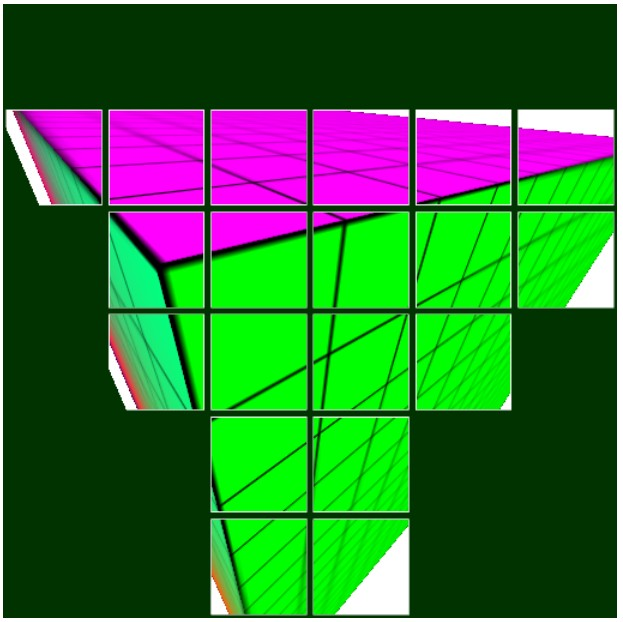
\includegraphics[width=.3\linewidth]{splat1.jpg}
  }
  \subfigure[$P_c M_c = P_s M_s$]{
    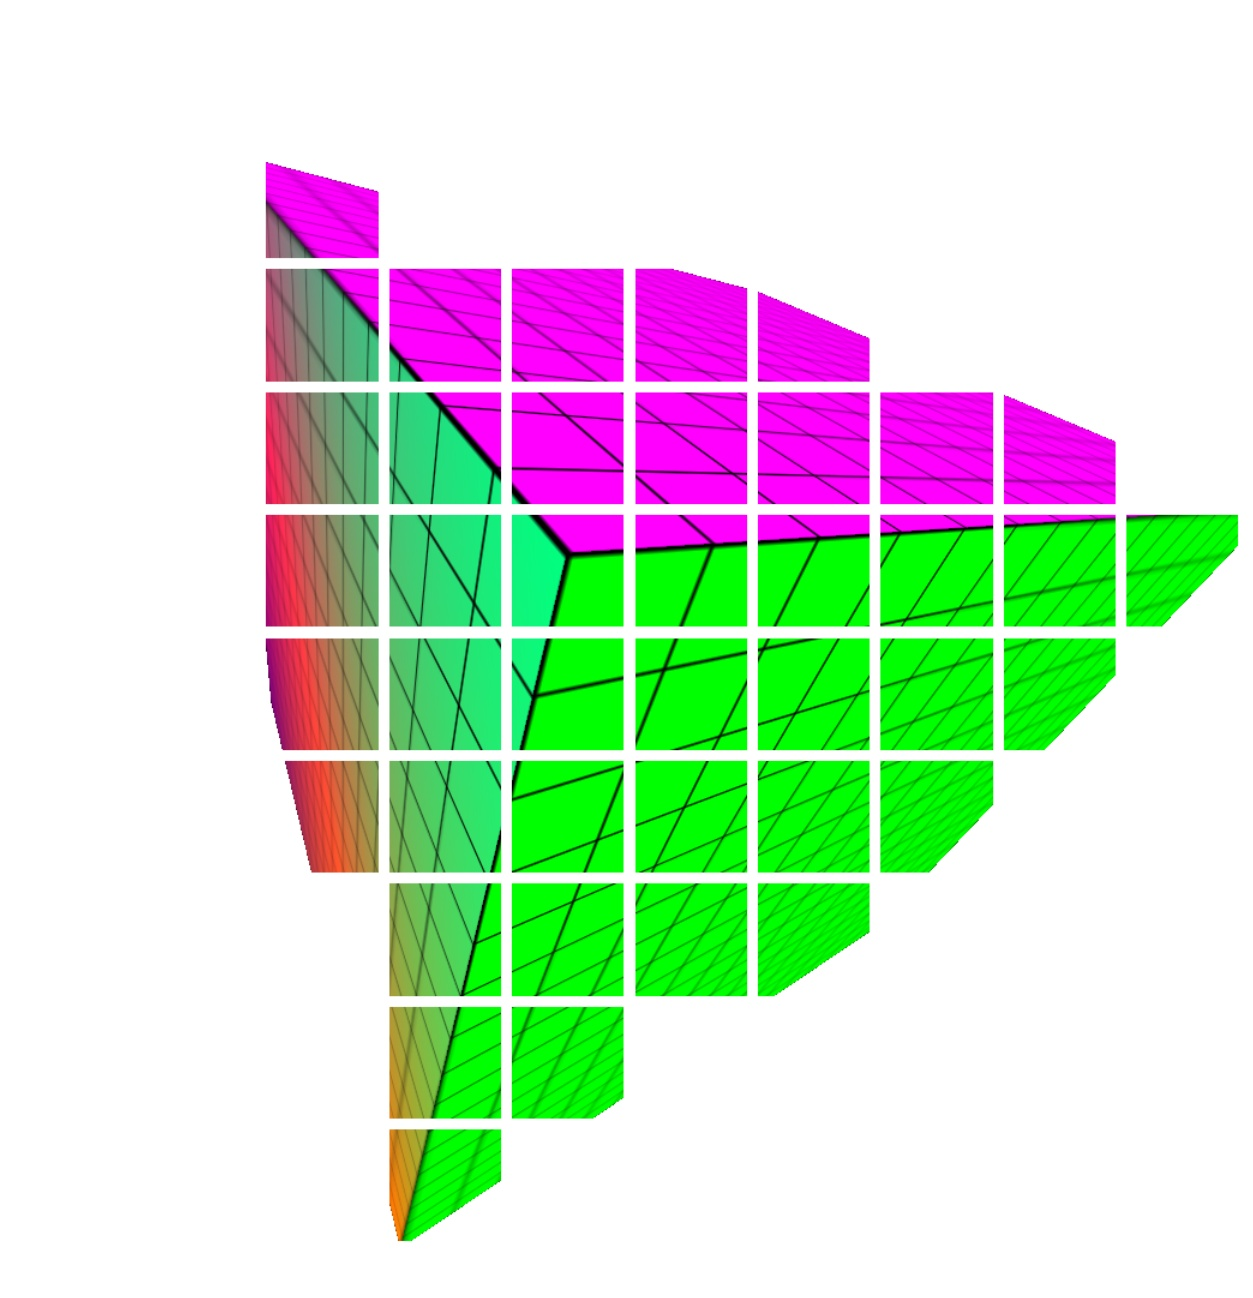
\includegraphics[width=.3\linewidth]{splat2.jpg}
  }
  \subfigure[$P_c M_c \neq P_s M_s$]{
    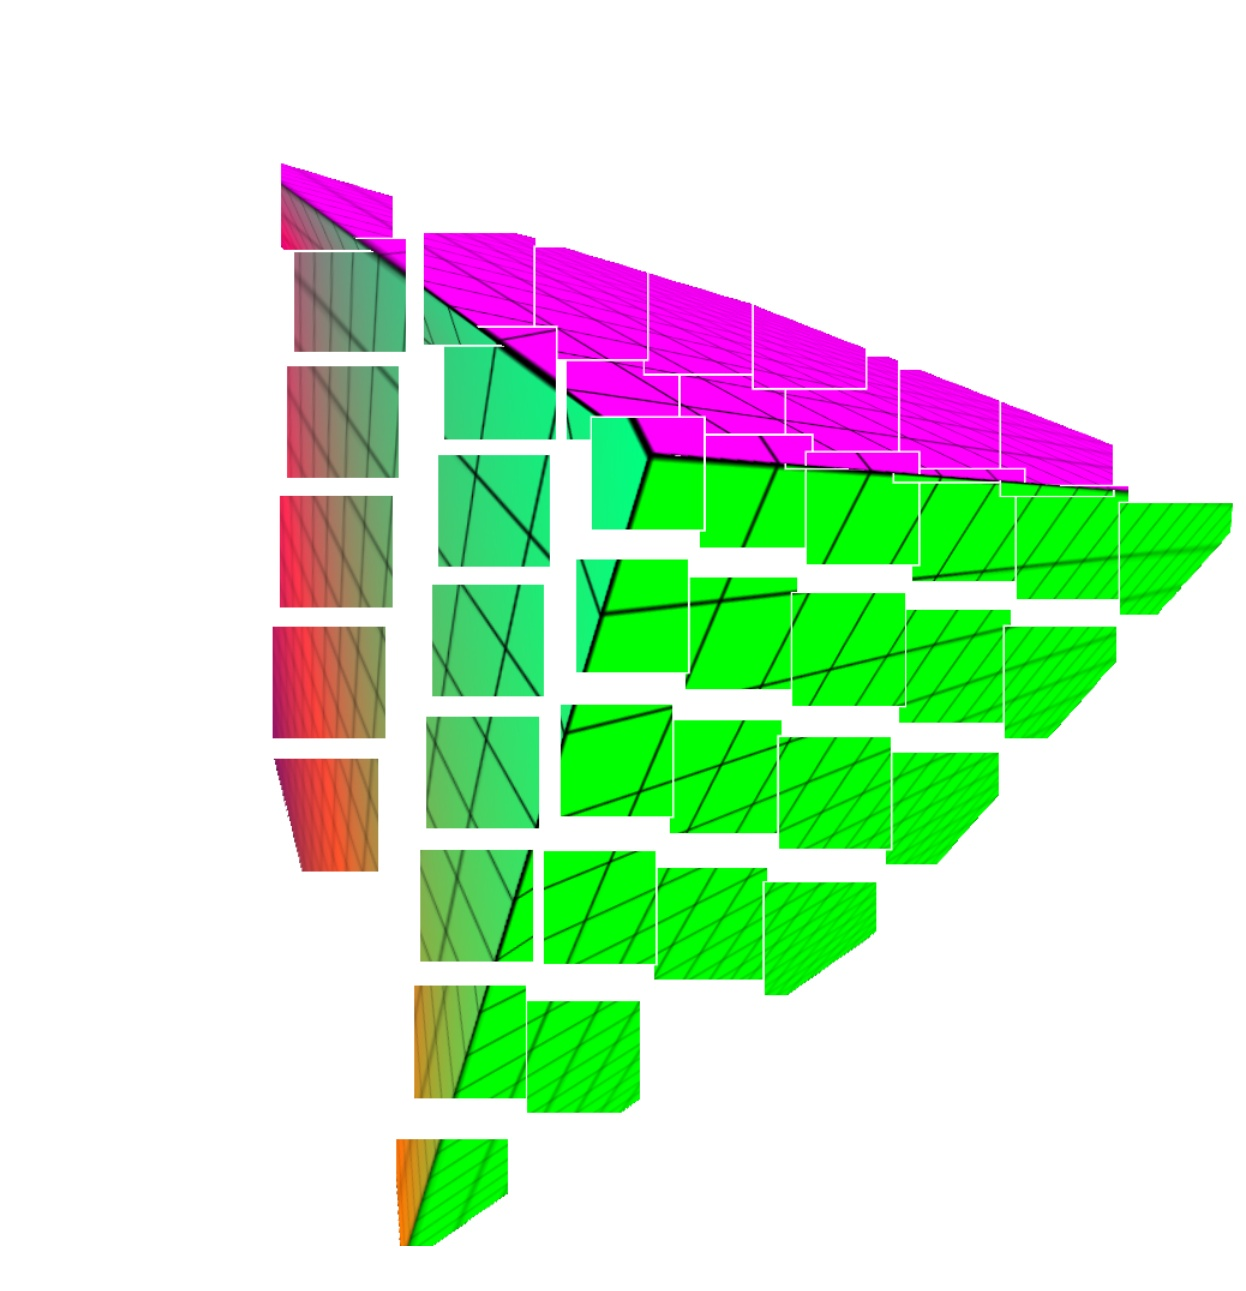
\includegraphics[width=.3\linewidth]{splat3.jpg}
  }
  \caption{\label{fig:LargeSplatsOnCorners}
           Splats for which depths are sampled on a planar region look nice on
  exactly this region, but contorted elsewhere, notice the corner and edges of
  the cube.}
\end{figure}

The problem illustrated in Figure~\ref{fig:LargeSplatsOnCorners}, is that the
geometry is far from planar, and our simple texture coordinate transformation
will produce the wrong result for the corresponding part of involved
splats. Some ways to remedy this is, \eg, to choose smaller (and more) splats,
detect the problem and discard such splats, or introduce more complex texture
transformations. Since the proxy geometry in principle is to be short-lived, and
only a temporary geometry to be rendered before the server-rendered image can be
receieved, we have chosen a combination of the first two alternatives. Note that
implementing a more sophisticated texture coordinate transformation may actually
amount to performing the same work as for more and smaller splats. Equivalently
, using more and smaller splats may be regarded as a better texture transform
implementation.


%-------------------------------------------------------------------------
\subsubsection{Other splat considerations}

{\color{red} ... samle avsnittene nedenfor og komprimere...}


%-------------------------------------------------------------------------
\subsubsection{Splat sizing}

Note that as soon as a given proxy model is transformed, each splat should
ideally be rendered into a number of client pixels according to the new splats
3D position. A splat transformed into view closer to the observer, should result
in more client fragments, and vice versa. To achieve this, we simply use the
vectors $\sv_{\Delta x}$ and $\sv_{\Delta y}$ from the previous section.
In addition to this, we scale the splats up a bit, typically with a factor 2, so
that they overlap. The benefit of this is that we can render rectangular
window-aligned splats on the client, without getting large uncovered areas when
interactively rotating and scaling the model quickly on the client.


%-------------------------------------------------------------------------
\subsubsection{Splat depth fragments}

For larger splats, covering many fragments, it makes sense to also compute and
use depth fragments in the client's fragment shader. This will improve the usage
of more proxy models simultaneously, since the risk of a splat with a not very
representative depth value covers another and better splat, is reduced. The
``intra-splat'' depth values can easily be fetched from the depth image, just as
the texture is looked up for color, with the same texture transformation. One
problem is that many thin clients may not support this, in WebGL, the ``frag
depth'' feature is an extension, which may not be supported everywhere.


%------------------------------------------------------------------------
\subsection{Splat set replacement algorithms}
\label{sec:proxyModelReplacement}

In this paper we mainly concern ourselves with proxy models defined as sets of
splats. Since each splat set is the product of one instance of a server-rendered
image, depth buffer and viewing parameters, it makes sense to retain more than
one such model on the client. By doing this, the client may combine them in
order to provide renderings for viewing parameters very different from the last
one received.

As soon as the client has a set of such proxy models, it will also need an
algorithm for replacing old models with new ones.  One can imagine a plethora of
{\em splat set replacement algorithms}, we have tested three approaches that all
retain a constant number of proxy models. The first algorithm is to replace the
one with a viewing direction differing the most from the newly received
model. The second simply replaces the oldest one in store. The third replaces a
proxy model $k$ if the replacement results in the following objective function
being reduced,
\[
  \text{coverage} =
  \sum_{i=1}^n 
    \sum_{j\neq i}^n 
      ( \angle(\textbf{camdir}_i, \textbf{camdir}_j )^2,
\]
where $n$ is the number of proxy models available and the model to be replaced
is the one that minimizes this after replacement.
%\textbf{droppe fra her: }
%\ie, if $\text{coverage}_k < \text{coverage}$, where
%\[
%  \text{coverage}_k =
%  \min_j
%  \sum_{i=1, i\neq j}^n 
%    ( \angle(\textbf{camdir}_i, \textbf{new\ camdir}_j )^2.
%\]
%\textbf{til hit?}
Here, $\textbf{camdir}$ is the direction in which the camera was looking for the
generation of that particular proxy model.  There are some issues to consider
with respect to panning and zooming that we will not discuss here due to the
limited space available.


%-------------------------------------------------------------------------
\subsection{Dynamic/heuristic method selection, depth compression, auto-tuning}
\label{sec:autoTuning}

Since the main purpose of the automatically generated proxy model is to
facilitate a client-rendered image while waiting for one from the server for
increased interactivity, it is important that the process of generating and
sending proxy model data from the server itself is not hold up more than
necessary. There are mainly three sources of delay for server-rendered images to
the client; high latency, low bandwidth, and slow server-rendering itself.

In the first case, it seems prudent to have a better proxy model on the client,
that can be used for longer time and for interactivity resulting in viewing
parameters deviating more from the last received server-rendered image. In the
two other cases, it is important for the proxy model generation/transmission to
be quicker, both in order to get the proxy model to the client and keep from
delaying the server-image more than necessary.

To take care of this, we have adopted an adaptive specification of
proxy model data from the server. This involves a more light-weight image (lossy
JPG-compression with adaptive quality control) while the user is interacting
with the client, as well as a reduced resolution of the depth buffer sent from
the server. Another possible form of auto-tuning is to let the client adaptively
choose the number of splats, stored number of proxy models, etc.

%See Figure~\ref{fig:adapativeProxyModels} for examples of low- and
%high-quality proxy models.
%\begin{figure}[htb]
%  \centering
%  \subfigure[Full png image,\newline full depth buffer]{
%    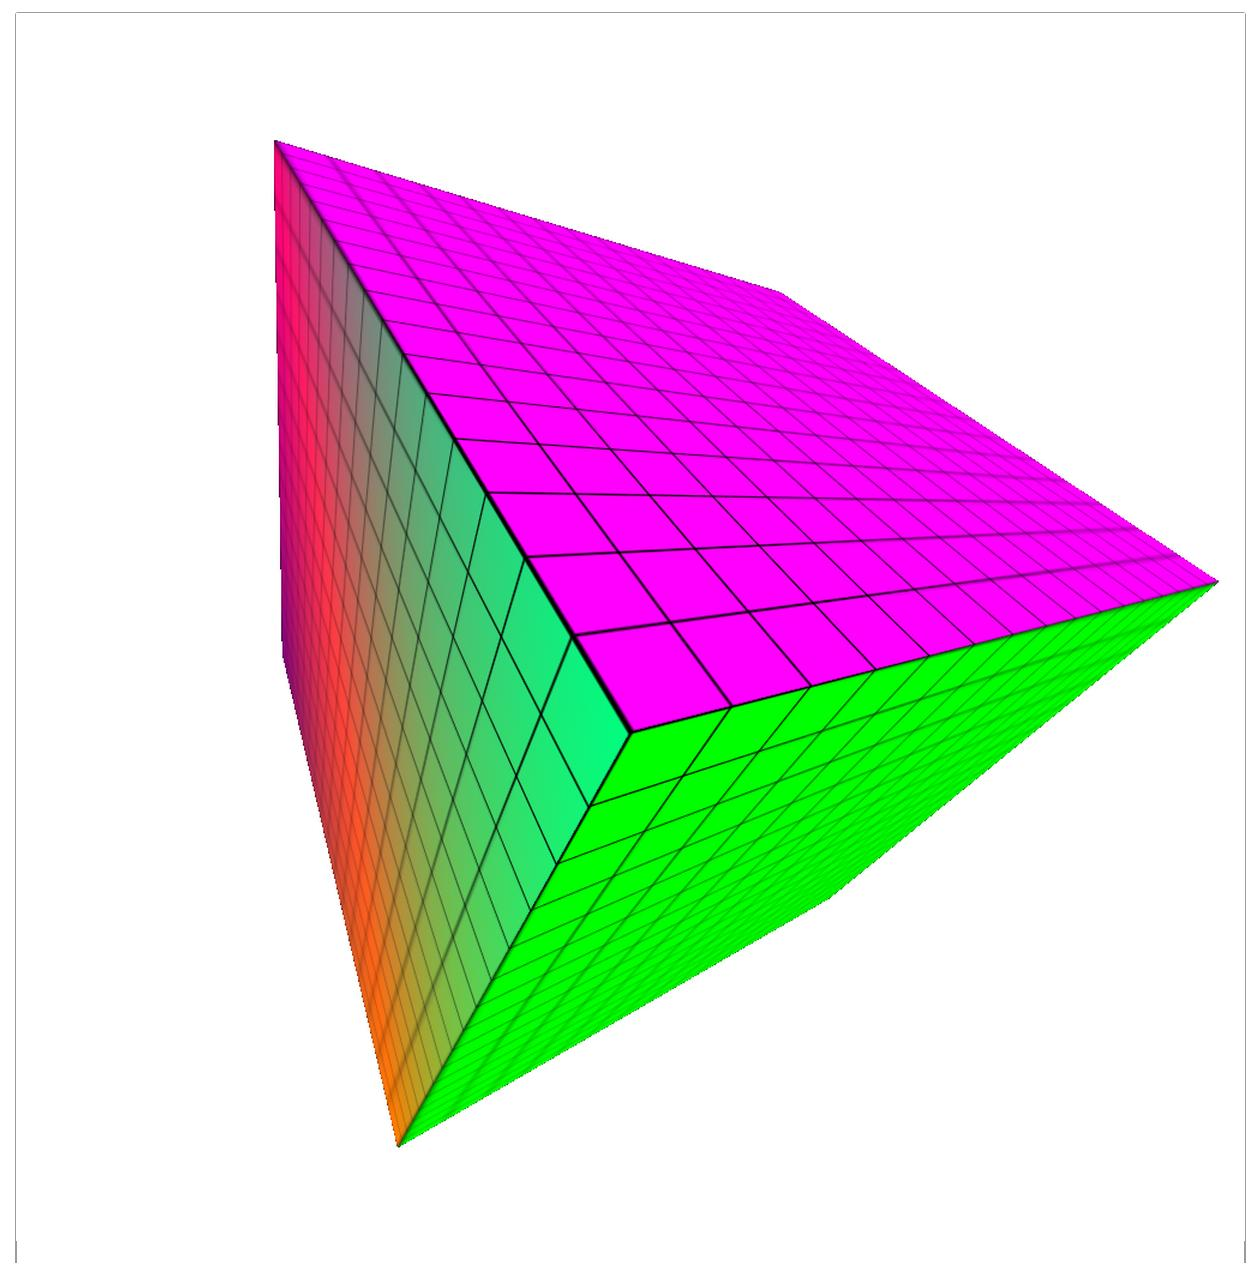
\includegraphics[width=.30\linewidth]{auto1.jpg}
%  }
%  \subfigure[Coarse jpg,\newline quality $q=0$]{
%    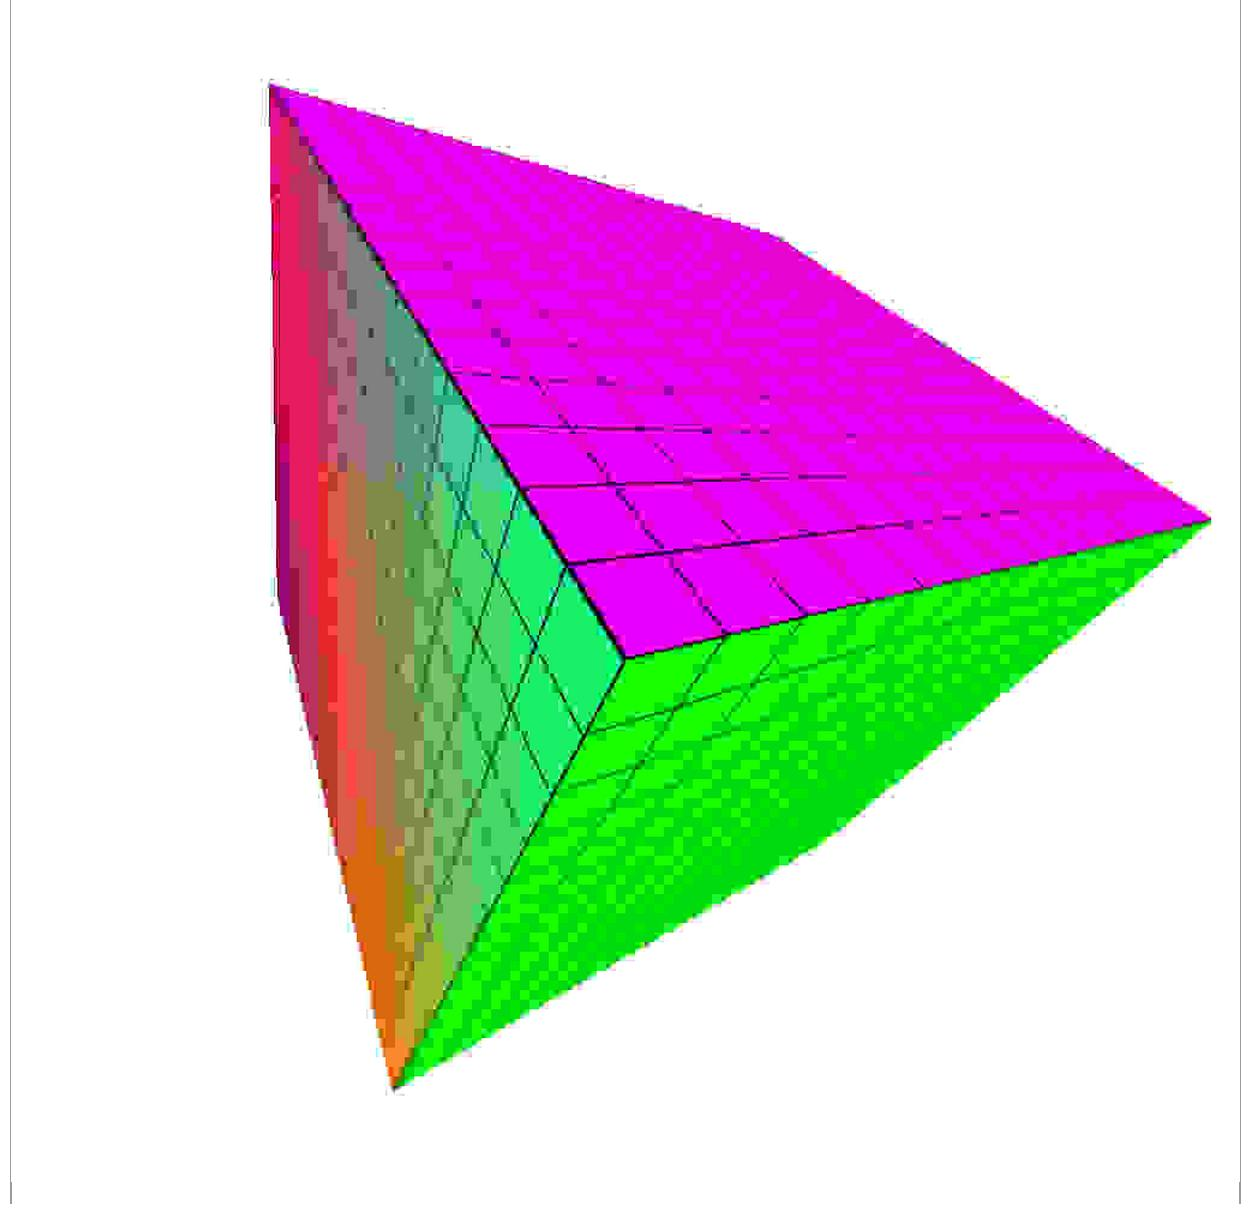
\includegraphics[width=.30\linewidth]{auto2.jpg}
%  }
%  \subfigure[Auto-proxy, trun-\newline cated depth data]{
%    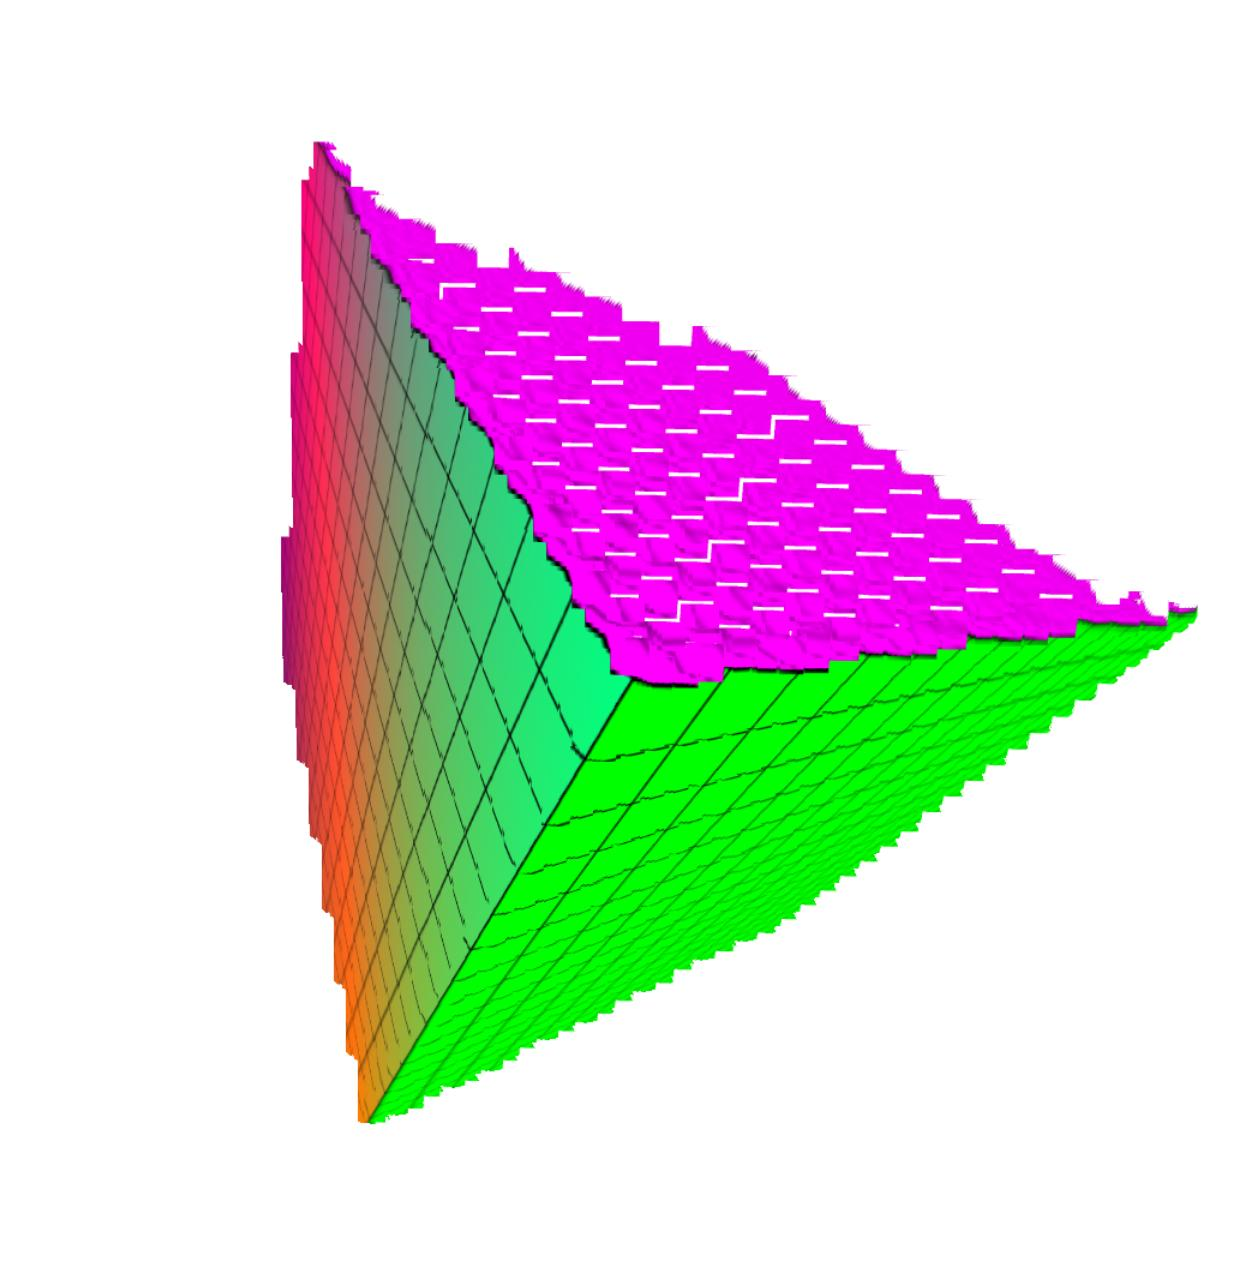
\includegraphics[width=.30\linewidth]{auto3.jpg}
%  }
%  \caption{\label{fig:adapativeProxyModels} Proxy models adaptively adjusted to
%           available bandwidth and server capacity. The server-rendered JPG
%           image adaptively selects a quality setting based on recorded
%           timings. Shown is the worst case, \texttt{quality}=0, (b) which is
%           the last step before switching to ``auto proxy'' (c). The auto-proxy
%           model shown displays artifacts caused both by the magenta surface
%           being almost parallel to the viewing direction at the moment of proxy
%           model recording, and by the non-smooth parts of the geometry
%           (corners). The number of splats is set low on purpose, and the depth
%           buffer size is reduced by a factor of $16^{-2} \approx 0.4\%$. \textbf{KRYMPE HER}}
%\end{figure}


%-------------------------------------------------------------------------
\section{Results and discussion}

We have tested the algorithms discussed in the Tinia framework, which is a
programming framework for setting up and managing a client/server based
interactive OpenGL-based visualization application, see~\cite{tinia}. As client
we use Google Chrome, the code is written in standard Javascript/WebGL.
The client communicatesover tcp/ip, using either http or
websockets, with a server running as an Apache module.

The automatic proxy geometry implementation in Tinia is fully invisible to the
application, meaning that all existing applications immediately will have the
feature available. Without Tinia, the algorithm is minimally intrusive in that
only the depth buffer will have to be added to the rendering output of the
application. We have tested the algorithm on several smaller test cases, but
also on a larger oil reservoir viewer, FRView, developed in the CloudViz
project, see~\cite{cloudviz}.

This viewer utilizes several GLSL shaders to render reservoir cells and
boundaries ({\em corner point grids}), tubular wells etc., and operates in
general on a geometric model that is not trivial to reduce in complexity. The
model is typically also very large, meaning that rendering the full model on a
thin client is prohibitive. With the automatic proxy geometry, we can obtain
interactive frame rates with a limited connection from a very lightweight client
to the server. For a comparison of a server-rendered image and a client-rendered
proxy model that is slightly rotated on the client, see again
Figure~\ref{fig:FRView}. {\color{red}In Figure~\ref{fig:FRView}~(a), the full
server-rendered image is shown, and in~(b) and~(c), a slightly (about 10
degrees) rotated proxy model is rendered on the client. In~(b), parameters are
chosen for best possible results, while in~(c), we want to highlight some
effects. For the latter, we have chosen a small number of non-overlapping
splats, which are also outlined. In this image, it is easy to spot areas not
well covered by any splats, and also some areas where the texture coordinate
transform $T$ does not produce optimal results.}


%-------------------------------------------------------------------------
\section{Conclusion and future work}

The single most attractive feature of such an automatic proxy geometry as
described, is exactly the automated generation. It means that problems with
downscaling, sending and rendering existing geometries is bypassed
altogether. The Tinia framework with which we have demonstrated this, is a
framework for setting up and managing a client/server based interactive OpenGL
based visualization application. The automatic proxy geometry implementation is
fully invisible to the application, meaning that all existing applications
immediately will have the feature available.

There are several directions in which we would like to follow up and improve
this concept, foremost of these are,
\begin{itemize}

\item \textbf{Proxy model replacement algorithms} The goal is to obtain a good view with
all relevant viewing parameters on the client, with the help of a minimal set of
proxy models.

%\item \textbf{Grid-based proxy geometry} Instead of a set of ``splats'', one can
%envision a spatially partioned grid, for instance containing a distance field,
%with the geometry as an iso-surface.

%\item \textbf{Client rendering with overlays} Items like, \eg, axis indicators,
%legends etc. that do not use the same view matrix as the main model could be
%rendered locally on the client, only. This will cancel some of the benefit
%connected to the automatic proxy model generation, though. \textbf{Nettopp av
%denne grunn kan kanskje dette vaere et punkt vi boer luke bort? Plassmangel
%ogsaa...}

\item \textbf{Depth compression} We have currently done a unsophisticated
truncation, but other approaches are possible,
like discussed in~\cite{DBLP:journals/tvcg/Lindstrom14}.

%\item \textbf{Improved auto-tuning} The auto-tuning discussed in
%Section~\ref{sec:autoTuning} should be extended to take not only server
%parameters (rendering quality, compression etc.) into account, but also the
%capabilities of various thin clients.

\item \textbf{Deferred shading} In addition to sending an image and a depth map
from the server, one could send also a normal map. (This can also be
reconstructed from the depth map on the client.) This would allow more advanced
shading on the client.

%\item \textbf{Stitching of 2.5D point clouds} As mentioned in
%Section~\ref{sec:prevWork}, we have considered but not experimented with
%stitching of depth maps from the server.

\end{itemize}




%-------------------------------------------------------------------------

%\bibliographystyle{eg-alpha}
\bibliographystyle{eg-alpha-doi}

\bibliography{egbibsample}

%-------------------------------------------------------------------------

\end{document}
